\documentclass[10pt,journal,compsoc, draftclsnofoot,onecolumn]{IEEEtran}

\usepackage{graphicx}
\usepackage{subcaption}
\usepackage{epstopdf}
\usepackage{amssymb}                                         
\usepackage{amsmath}                                         
\usepackage{amsthm}                                          

\usepackage{alltt}                                           
\usepackage{float}
\usepackage{color}
\usepackage{url}

\usepackage{balance}
\usepackage{enumitem}
\usepackage{pstricks, pst-node}

\usepackage[margin=0.75in]{geometry}
\geometry{textheight=8.5in, textwidth=6in}

\newcommand{\cred}[1]{{\color{red}#1}}
\newcommand{\cblue}[1]{{\color{blue}#1}}
\usepackage{geometry}

\usepackage{hyperref}
\usepackage{fancyvrb}
\usepackage{color}
\usepackage[latin1]{inputenc}


\makeatletter
\def\PY@reset{\let\PY@it=\relax \let\PY@bf=\relax%
    \let\PY@ul=\relax \let\PY@tc=\relax%
    \let\PY@bc=\relax \let\PY@ff=\relax}
\def\PY@tok#1{\csname PY@tok@#1\endcsname}
\def\PY@toks#1+{\ifx\relax#1\empty\else%
    \PY@tok{#1}\expandafter\PY@toks\fi}
\def\PY@do#1{\PY@bc{\PY@tc{\PY@ul{%
    \PY@it{\PY@bf{\PY@ff{#1}}}}}}}
\def\PY#1#2{\PY@reset\PY@toks#1+\relax+\PY@do{#2}}

\expandafter\def\csname PY@tok@gd\endcsname{\def\PY@tc##1{\textcolor[rgb]{0.63,0.00,0.00}{##1}}}
\expandafter\def\csname PY@tok@gu\endcsname{\let\PY@bf=\textbf\def\PY@tc##1{\textcolor[rgb]{0.50,0.00,0.50}{##1}}}
\expandafter\def\csname PY@tok@gt\endcsname{\def\PY@tc##1{\textcolor[rgb]{0.00,0.25,0.82}{##1}}}
\expandafter\def\csname PY@tok@gs\endcsname{\let\PY@bf=\textbf}
\expandafter\def\csname PY@tok@gr\endcsname{\def\PY@tc##1{\textcolor[rgb]{1.00,0.00,0.00}{##1}}}
\expandafter\def\csname PY@tok@cm\endcsname{\let\PY@it=\textit\def\PY@tc##1{\textcolor[rgb]{0.25,0.50,0.50}{##1}}}
\expandafter\def\csname PY@tok@vg\endcsname{\def\PY@tc##1{\textcolor[rgb]{0.10,0.09,0.49}{##1}}}
\expandafter\def\csname PY@tok@m\endcsname{\def\PY@tc##1{\textcolor[rgb]{0.40,0.40,0.40}{##1}}}
\expandafter\def\csname PY@tok@mh\endcsname{\def\PY@tc##1{\textcolor[rgb]{0.40,0.40,0.40}{##1}}}
\expandafter\def\csname PY@tok@go\endcsname{\def\PY@tc##1{\textcolor[rgb]{0.50,0.50,0.50}{##1}}}
\expandafter\def\csname PY@tok@ge\endcsname{\let\PY@it=\textit}
\expandafter\def\csname PY@tok@vc\endcsname{\def\PY@tc##1{\textcolor[rgb]{0.10,0.09,0.49}{##1}}}
\expandafter\def\csname PY@tok@il\endcsname{\def\PY@tc##1{\textcolor[rgb]{0.40,0.40,0.40}{##1}}}
\expandafter\def\csname PY@tok@cs\endcsname{\let\PY@it=\textit\def\PY@tc##1{\textcolor[rgb]{0.25,0.50,0.50}{##1}}}
\expandafter\def\csname PY@tok@cp\endcsname{\def\PY@tc##1{\textcolor[rgb]{0.74,0.48,0.00}{##1}}}
\expandafter\def\csname PY@tok@gi\endcsname{\def\PY@tc##1{\textcolor[rgb]{0.00,0.63,0.00}{##1}}}
\expandafter\def\csname PY@tok@gh\endcsname{\let\PY@bf=\textbf\def\PY@tc##1{\textcolor[rgb]{0.00,0.00,0.50}{##1}}}
\expandafter\def\csname PY@tok@ni\endcsname{\let\PY@bf=\textbf\def\PY@tc##1{\textcolor[rgb]{0.60,0.60,0.60}{##1}}}
\expandafter\def\csname PY@tok@nl\endcsname{\def\PY@tc##1{\textcolor[rgb]{0.63,0.63,0.00}{##1}}}
\expandafter\def\csname PY@tok@nn\endcsname{\let\PY@bf=\textbf\def\PY@tc##1{\textcolor[rgb]{0.00,0.00,1.00}{##1}}}
\expandafter\def\csname PY@tok@no\endcsname{\def\PY@tc##1{\textcolor[rgb]{0.53,0.00,0.00}{##1}}}
\expandafter\def\csname PY@tok@na\endcsname{\def\PY@tc##1{\textcolor[rgb]{0.49,0.56,0.16}{##1}}}
\expandafter\def\csname PY@tok@nb\endcsname{\def\PY@tc##1{\textcolor[rgb]{0.00,0.50,0.00}{##1}}}
\expandafter\def\csname PY@tok@nc\endcsname{\let\PY@bf=\textbf\def\PY@tc##1{\textcolor[rgb]{0.00,0.00,1.00}{##1}}}
\expandafter\def\csname PY@tok@nd\endcsname{\def\PY@tc##1{\textcolor[rgb]{0.67,0.13,1.00}{##1}}}
\expandafter\def\csname PY@tok@ne\endcsname{\let\PY@bf=\textbf\def\PY@tc##1{\textcolor[rgb]{0.82,0.25,0.23}{##1}}}
\expandafter\def\csname PY@tok@nf\endcsname{\def\PY@tc##1{\textcolor[rgb]{0.00,0.00,1.00}{##1}}}
\expandafter\def\csname PY@tok@si\endcsname{\let\PY@bf=\textbf\def\PY@tc##1{\textcolor[rgb]{0.73,0.40,0.53}{##1}}}
\expandafter\def\csname PY@tok@s2\endcsname{\def\PY@tc##1{\textcolor[rgb]{0.73,0.13,0.13}{##1}}}
\expandafter\def\csname PY@tok@vi\endcsname{\def\PY@tc##1{\textcolor[rgb]{0.10,0.09,0.49}{##1}}}
\expandafter\def\csname PY@tok@nt\endcsname{\let\PY@bf=\textbf\def\PY@tc##1{\textcolor[rgb]{0.00,0.50,0.00}{##1}}}
\expandafter\def\csname PY@tok@nv\endcsname{\def\PY@tc##1{\textcolor[rgb]{0.10,0.09,0.49}{##1}}}
\expandafter\def\csname PY@tok@s1\endcsname{\def\PY@tc##1{\textcolor[rgb]{0.73,0.13,0.13}{##1}}}
\expandafter\def\csname PY@tok@sh\endcsname{\def\PY@tc##1{\textcolor[rgb]{0.73,0.13,0.13}{##1}}}
\expandafter\def\csname PY@tok@sc\endcsname{\def\PY@tc##1{\textcolor[rgb]{0.73,0.13,0.13}{##1}}}
\expandafter\def\csname PY@tok@sx\endcsname{\def\PY@tc##1{\textcolor[rgb]{0.00,0.50,0.00}{##1}}}
\expandafter\def\csname PY@tok@bp\endcsname{\def\PY@tc##1{\textcolor[rgb]{0.00,0.50,0.00}{##1}}}
\expandafter\def\csname PY@tok@c1\endcsname{\let\PY@it=\textit\def\PY@tc##1{\textcolor[rgb]{0.25,0.50,0.50}{##1}}}
\expandafter\def\csname PY@tok@kc\endcsname{\let\PY@bf=\textbf\def\PY@tc##1{\textcolor[rgb]{0.00,0.50,0.00}{##1}}}
\expandafter\def\csname PY@tok@c\endcsname{\let\PY@it=\textit\def\PY@tc##1{\textcolor[rgb]{0.25,0.50,0.50}{##1}}}
\expandafter\def\csname PY@tok@mf\endcsname{\def\PY@tc##1{\textcolor[rgb]{0.40,0.40,0.40}{##1}}}
\expandafter\def\csname PY@tok@err\endcsname{\def\PY@bc##1{\setlength{\fboxsep}{0pt}\fcolorbox[rgb]{1.00,0.00,0.00}{1,1,1}{\strut ##1}}}
\expandafter\def\csname PY@tok@kd\endcsname{\let\PY@bf=\textbf\def\PY@tc##1{\textcolor[rgb]{0.00,0.50,0.00}{##1}}}
\expandafter\def\csname PY@tok@ss\endcsname{\def\PY@tc##1{\textcolor[rgb]{0.10,0.09,0.49}{##1}}}
\expandafter\def\csname PY@tok@sr\endcsname{\def\PY@tc##1{\textcolor[rgb]{0.73,0.40,0.53}{##1}}}
\expandafter\def\csname PY@tok@mo\endcsname{\def\PY@tc##1{\textcolor[rgb]{0.40,0.40,0.40}{##1}}}
\expandafter\def\csname PY@tok@kn\endcsname{\let\PY@bf=\textbf\def\PY@tc##1{\textcolor[rgb]{0.00,0.50,0.00}{##1}}}
\expandafter\def\csname PY@tok@mi\endcsname{\def\PY@tc##1{\textcolor[rgb]{0.40,0.40,0.40}{##1}}}
\expandafter\def\csname PY@tok@gp\endcsname{\let\PY@bf=\textbf\def\PY@tc##1{\textcolor[rgb]{0.00,0.00,0.50}{##1}}}
\expandafter\def\csname PY@tok@o\endcsname{\def\PY@tc##1{\textcolor[rgb]{0.40,0.40,0.40}{##1}}}
\expandafter\def\csname PY@tok@kr\endcsname{\let\PY@bf=\textbf\def\PY@tc##1{\textcolor[rgb]{0.00,0.50,0.00}{##1}}}
\expandafter\def\csname PY@tok@s\endcsname{\def\PY@tc##1{\textcolor[rgb]{0.73,0.13,0.13}{##1}}}
\expandafter\def\csname PY@tok@kp\endcsname{\def\PY@tc##1{\textcolor[rgb]{0.00,0.50,0.00}{##1}}}
\expandafter\def\csname PY@tok@w\endcsname{\def\PY@tc##1{\textcolor[rgb]{0.73,0.73,0.73}{##1}}}
\expandafter\def\csname PY@tok@kt\endcsname{\def\PY@tc##1{\textcolor[rgb]{0.69,0.00,0.25}{##1}}}
\expandafter\def\csname PY@tok@ow\endcsname{\let\PY@bf=\textbf\def\PY@tc##1{\textcolor[rgb]{0.67,0.13,1.00}{##1}}}
\expandafter\def\csname PY@tok@sb\endcsname{\def\PY@tc##1{\textcolor[rgb]{0.73,0.13,0.13}{##1}}}
\expandafter\def\csname PY@tok@k\endcsname{\let\PY@bf=\textbf\def\PY@tc##1{\textcolor[rgb]{0.00,0.50,0.00}{##1}}}
\expandafter\def\csname PY@tok@se\endcsname{\let\PY@bf=\textbf\def\PY@tc##1{\textcolor[rgb]{0.73,0.40,0.13}{##1}}}
\expandafter\def\csname PY@tok@sd\endcsname{\let\PY@it=\textit\def\PY@tc##1{\textcolor[rgb]{0.73,0.13,0.13}{##1}}}

\def\PYZbs{\char`\\}
\def\PYZus{\char`\_}
\def\PYZob{\char`\{}
\def\PYZcb{\char`\}}
\def\PYZca{\char`\^}
\def\PYZam{\char`\&}
\def\PYZlt{\char`\<}
\def\PYZgt{\char`\>}
\def\PYZsh{\char`\#}
\def\PYZpc{\char`\%}
\def\PYZdl{\char`\$}
\def\PYZti{\char`\~}
% for compatibility with earlier versions
\def\PYZat{@}
\def\PYZlb{[}
\def\PYZrb{]}
\makeatother


\begin{document}

\title{Project Hand Off
    \\3D Object Pose Tracking for Robotics Grasping
    \\Lux Vision
    \\CS 463 | Spring 2019}
\author{Connor Campbell, Chase McWhirt, Jiawei Mo}

\maketitle

\begin{abstract}
The report explains many details regarding the Robotic Vision project.
It acts as a depiction of the Robotic Vision project, including triumphs and struggles.
Many of the changes made are detailed, as well as a basic understanding of the machine learning models implemented.

\end{abstract}

\IEEEdisplaynontitleabstractindextext
\IEEEpeerreviewmaketitle

\newpage
\tableofcontents

\newpage
\section{Introduction}
%---------Who requested it? \\
%---------Why was it requested? \\
%---------What is its importance? \\
%---------Who was/were your client(s)? \\
%---------Who are the members of your team? \\
%---------What were their roles? \\
%---------What was the role of the client(s)? (I.e., did they supervise only, or did they participate in doing development) \\

\noindent
The goal of this project was find and implement a method to identify a robot arm with 90\% accuracy.
This metric was met initially with an artificial neural network then with a convolutional neural network.
Our client, Cindy Grimm, wants this project developed to fit into her larger project.
The larger project is to create a way for people to remotely access the arm and perform experiments in the hopes of improving hand grasping mechanics.
However, in order for the arm to function in this way autonomously, it needs to have a trained vision system to guide its movements. \\

\noindent
Connor Campbell, Chase McWhirt, and Jiawei Mo all created different machine learning implementations to be able to identify the arm based on 640x480 pixel frames.
Respectively, they implemented the artificial neural network, support vector machine, and K-means clustering implementations.
Connor represented the group as team leader, divided data in nearest neighbor groupings, and helped ensure quality documentation.
Chase organized and kept track of project goals, created extra scripts to be used on all implementations, and wrote group emails.
Jiawei researched computer vision topics that supported implementations, implemented an alternative, deep-learning convolutional neural network, and intiated many of the group reports.
Cindy's role was typically to supervise but she shared knowledge when requested.


\newpage
\section{Requirements}
%---------Include newest copy of the requirements document. Be sure to include the CHANGE TABLE showing updates to original requirements. \\
%---------Update: Final Gantt Chart as a record of what happened when.

\begin{abstract}
As robots and artificial intelligence become increasingly important in the modern age, they will need to be able to interact with their environment on their own, and computer vision is an integral part of a robot's understanding of its surroundings.
Oregon State University's robotics department has an ongoing project attempting to improve computer vision, and this Capstone project is aimed at furthering that goal.
Specifically, this Capstone project will be the culmination of implementing various dynamic masking techniques that can be executed in real time.
\end{abstract}

\subsection{Table of Changes}
\begin{center}
\begin{tabular}{|p{0.3\linewidth}|p{0.3\linewidth}|p{0.3\linewidth}|p{0.2\linewidth}|}
\hline
Section & Original & New \\ [0.5ex]
\hline\hline

Functional Requirements
&
Images grouped based on data for arm's specific pose.
Images will come in stereoscopic pairs.
&
Images roughly based on pose, based on time stamp from video the images came from.
Images are individual, monoscopic frames.
\\ \hline

Performance Requirements
&
Preferred 80\% accuracy on best method.
&
Best method should have an average of 90\% accuracy in the area with the arm within prediction masks.
\\ \hline

Verification
&
Preferred 80\% accuracy on best method.
False negatives are worse than false positives.
&
Best method should have an average of 90\% accuracy in the area with the arm within prediction masks.
False negative and false positives are counted the same.
\\ \hline

Definitions
&
N/A
&
Added definition for Support Vector Machine.
\\ \hline
\end{tabular}
\end{center}

\subsection{Purpose}
This document will define the goals given by the client.
The goals will include specific tasks that can be accomplished by a single person.
These tasks will be defined in such a way that they are easily distributed among the group members.
Tasks will also effectively be verifiable.

\subsection{Overview}
\subsubsection{Product Perspective}
The project is only a piece of a much larger project.
The larger project is a robotic grasping problem.
Oregon State University has a robotic arm that should be able to grasp and manipulate an object within a specific environment.
The environment will be a box containing the desired object for manipulation, the robotic arm, a single light source, and two cameras placed on adjacent corners of the ceiling.
This particular robotic arm has no tactile sense.
Thus, it must be able to understand the entire environment with only optical input.
The project discussed in this document is geared to solving the problem of handling optical input.
The current code behind this functionality is able to understand its environment by finding cross sections within its two camera inputs.
This effectively gives the robot stereo vision.
However, its sense of objects is extremely limited.
The code behind the robotic arm attempts to create a mask over important objects in the scene.
This functionality expects uniform color though.
Since the environment only contains a single light source, it is essentially impossible for an important object to be uniformly colored.
Light diffusion will make an object appear covered in a wide variety of shades.
If there were multiple light sources, this effect could be decreased.
However, since an object is going to be manipulated, creating perfect lighting conditions is highly unrealistic.

\noindent
It should be noted that these functions will primarily be used by the University's robotics research team.
They won't be robust enough for complex, real world applications, but are rather meant to be a step forward for future research.

\subsubsection{Product Functions}
In order to solve the problem of inconsistent light sources, this project will have to create and execute a more dynamic method of image masking to accurately identify the object.
The client has discussed multiple possible approaches to do this, but is not sure which method will work best.
There will be three different implementations attempted and these will be tested against a straw man implementation.
The best implementation measured against the straw man will become the final product.
This project will only attempt to find the best masking function for identifying the robotic arm itself.
As stretch goals, the best method found in the main project will be implemented to mask the object the robotic arm will grasp.
As a final stretch goal, both masking methods will be verified as compatible with each other.

\subsubsection{Constraints}
This phase is a part of a big project.
Our group is to undertake only the lighting changes during object grasping.
As such, it will need to interact appropriately with the rest of the project.
Since this program is meant to replace an older identification system, it will be ideal for the inputs and outputs to be similar, in order to minimize the need for adjustments to the rest of the project.

\subsection{System Requirements}
\subsubsection{Functional requirements}
To begin, this project will be based on monoscopic images and time stamps that our client has gathered.
These images will be of the robotic arm in various poses, and will be used both for training and testing the algorithms.
The initial straw man will be determined by simply running a k-means clustering over all of the data to determine a color range to look for.
Next, the images will be roughly grouped based on the arm's pose.
Specifically, the images will be still frames from a video of the arm moving, and the groups will be based on the time stamps for the images.
Each group will have its own version of each of the three methods.
The three methods include another k-means clustering (though over a single group as opposed to all of the data), neural networks, and support vector machines.

\subsubsection{Performance requirements}
The goal is for the best of the three methods to replace part of the larger project's current system.
As such, it should label around 90\% of the pixels in a region around the arm correctly as either part of the arm or not. This region will be defined as the smallest rectangle containing the entirety of the arm for the given image

\subsection {Verification}
Implementation effectiveness can be measured in two distinct ways.
First, it can be measured against a designated "truth" defined when images were manually masked.
Each pixel will fall into four groups.
True positives are when the program correctly identifies a pixel as part of the robot arm.
True negatives are when the pixel is correctly labeled as not part of the arm.
False positives are when a pixel is labeled as part of the arm and it is not incorrect.
Finally, false negatives are masking a pixel as not part of the arm and being incorrect.
The client has stated a desired accuracy of 90\% or more in the relevant parts of the image.

\noindent
The other way to verify each implementation is whether or not it is more effective than the straw man.
If it is less effective, the implementation fails.
If it is more effective, it passes.
It is possible to measure how much more effective the implementation is over the straw man.
For example, if the straw man has 40\% of all true positives and implementation x has 80\% of all true positives, implementation x is twice as effective at defining true positives than the straw man.
This concept will be important for defining how successful any implementation is.

\subsection{Definitions}
\begin{itemize}
\item K-means Clustering - An algorithm that involves dividing a group of data points into smaller groups such that each point is in the group with the group average most similar to it.

\item Mask - An overlay defining a set of pixels as a unique object.
Applying a mask over an object is the main goal of the project.

\item Neural Network - A form of machine learning designed to mimic the activity of organic brains by simulating neurons firing in order. This can be simplified as a multiplying a series of matrices to the input.

\item Stereo Vision - Also known as binocular vision, this is the mechanic of taking two images taken from different angles and defining a perceived depth.

\item Straw Man - In this instance, a straw man is an implementation that is expected to under perform.
An extreme general approach is tested and measured.
It then acts as a baseline metric to compare to other implementations.

\item Support Vector Machine - A supervised learning model with classification and regression analysis.
For this project, data has binary classification (part of the arm or not part of the arm).
Thus, a linear regression analysis was chosen.

\end{itemize}

\subsection{Gantt Chart of Reality}
\begin{figure}[H]
  \begin{center}
    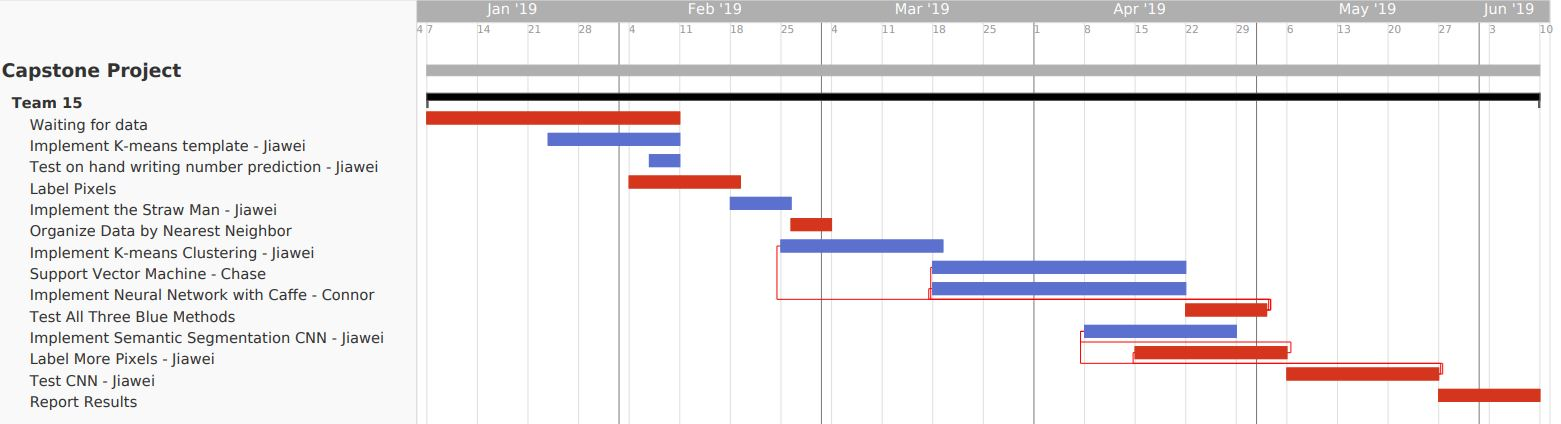
\includegraphics[width=1.\textwidth]{update_chart.JPG}
  \end{center}
  \caption{Final Gantt Chart}
\end{figure}


\newpage
\section{Design}
%---------Include newest copy of the design document. Be sure to include the CHANGE TABLE showing updates to original requirements.

\begin{abstract}
Robotic vision is an advanced topic that requires proper planning and consideration before attempting. In this project, a computer will be taught to recognize a robotic arm in an image by first narrowing down the region of the image it is likely in, then scanning the area with a neural networks. Different solutions as well as technologies used for achieving them are discussed.
\end{abstract}

\subsection{Table of Changes}
\begin{center}
\begin{tabular}{|p{0.3\linewidth}|p{0.3\linewidth}|p{0.3\linewidth}|}
\hline
Section & Original & New \\ [0.5ex]
\hline\hline

Summary
&
Groups based on data for arm pose.
Strict description of neural network structure.
&
Groups roughly based on pose base on time stamps for images.
Neural network structure can be experimented with.
\\ \hline

Glossary
&
Mentions of Gimp and Caffe
&
Gimp and Caffe were removed, as we used Photoshop and FANN instead.
Definition for Support Vector Machine provided
\\ \hline

Glossary
&
Added support vector machines and matplotlib.
&
Added a barebones definition of support vector machines.
Also described matplotlib, the Python alternative to OpenCV.
\\ \hline

Stakeholders
&
Our teacher's assistant was Wesley Alexis
&
Our teacher's assistant is now Omeed Habibelahian
\\ \hline

Design Concerns
&
No mention of desired platform.
&
The platform the project is done on does not matter to the client.
\\ \hline

Design Aspects - Support Vector Machine
&
(Nothing about support vector machines.)
&
A new section containing information about support vector machines, the library used, and notes about turning an image into a prediction mask.
\\ \hline

Design Aspects - Neural Network API
&
We planned to use the Caffe framework
&
Used FANN Library instead
\\ \hline

Design Aspects - Qualifying Data
&
We planned to use Gimp.
&
We used Photoshop.
Data only collected from the areas of images immediately surrounding the arm.
\\ \hline

\end{tabular}
\end{center}

\begin{center}
\begin{tabular}{|p{0.3\linewidth}|p{0.3\linewidth}|p{0.3\linewidth}|}
\hline
Section & Original & New \\ [0.5ex]
\hline\hline

Design Aspects - Input Images
&
Running on Python with package called OpenCV.
&
OpenCV is used in Neural Network solution by coding with C++. Right now, Kmeans use numpy package to read images as matrices to process.
\\ \hline

Design Aspects - Kmeans Learning
&
N/A
&
Using sklearn package to build up learning model and prediction function. The packge is available on Python official website.
\\ \hline

Show Masks During Running - Kmeans
&
N/A
&
Using matplotlib packges to pop the generated masks to a window for testing. It is available from Python official site.
\\ \hline

Saving Generated Masks - Kmeans
&
N/A
&
Using misc from scipy package to save generated masks in .png format. It is available from Python official site.
\\ \hline

Conclusion
&
Ideal accuracy 80-90\%
&
Accuracy should be 90\% between the predictions masks only within the arm's bounds.
\\ \hline
\end{tabular}
\end{center}

\subsection{Introduction}
\subsubsection{Purpose}
The goal of this document is provide a clear path of execution to stakeholders about how this product development project will reach completion.
It should ensure that the client, the instructors, and the students all understand how this project will be completed.

\subsubsection{Scope}
This document will describe various technologies, design choices, and a measurable progress checklist that will guide the rest of this product development project.

\subsubsection{Context}
This document is being written not only as a road map for our stakeholder, but also for our teachers and teachers' assistants to follow.
The project must be feasible to complete to the specifications by March 22, the end of Winter term, 2019.
If the project isn't completed by this time, there is only minimal flexibility available before the Oregon State Engineering Expo on May 17.

\subsubsection{Summary}
The end goal of this project is to create a software that will accurately identify a robotic arm in a given image.
Several possible solution plans have been created with the help of the client.
The client is going to take many photos of the robotic arm.
A straw man solution will be generated by running a k-means clustering method on all of the images, which will yield a naive method for identifying parts of the robotic arm.
This will act as a base line: the other solutions will be considered successful if they prove to be better than the straw man solution.

\noindent
The images will be categorized roughly based on the robotic arm's pose.
The images will be frames from a video of the arm in motion, and the groups will be based on the time stamps of each image.
The other solutions will work using those categorizations.

\noindent
The first possible solution is to run k-means on each of the pose groups.
The other solution is to train small neural networks on each subgroup. The client suggested two hidden layers of eight nodes each for these networks, though the exact structure will be experimented with.
With three inputs and two outputs, it should not be too time consuming to train each neural network.
10\% of the data will be set aside to test the effectiveness of each neural network.

\noindent
Finally, as a backup plan, if none of the solutions performs better than the straw man (or perhaps to run alongside the three solutions regardless) a neural network will be trained on all of the data (without pose nearest neighbor groupings) to see if it can get better results.
This will also be tested with 10\% of the data as well.

\subsection{Glossary}
\textbf{HSV}: Stands for Hue, Saturation and Value. It is a color model used for defining colors in computer graphics.

\noindent
\textbf{K-means clustering}: A method of dividing a large set of data into smaller portions based on where the data points tend to cluster.

\noindent
\textbf{Support Vector Machine}: A supervised learning model with classification and regression analysis.
For this project, data has binary classification (part of the arm or not part of the arm).
Thus, a linear regression analysis was chosen.

\noindent
\textbf{Neural Network}: A type of machine learning algorithm that can be trained to solve a variety of problems. Several layers of nodes simulate the firing of neurons.

\noindent
\textbf{OpenCV}: An open source library for computer vision field.
It was initially released in 2000 and written in C/C++.
It supports various operating system and has interfaces for different programming languages, including Python, C and C++. The latest version is 4.0.0.

\noindent
\textbf{matplotlib.image}: A Python alternative to OpenCV.
Used purely to open images as a list of RGB values and save lists of RGB values as images (at least by the SVM implementation).

\noindent
\textbf{RBG}: Stands for Red, Blue and Green. A different color model.

\subsection{Stakeholders and Design Concerns}
There are three primary stakeholders vested in this project.
The first is the client and sponsor, Cindy Grimm, whose primary concerns are completion of the project within particular specifications.
There are also the instructors, Kevin McGrath and Kirsten Winters, and the teaching assistant assigned to this project Omeed Habibelahian.
Their primary concerns are upholding mandatory standards of practice and quality assurance.
While in the context of the class, we should consider all stakeholders and concerns, this document will focus on the client's concerns.
The platform in which this project is done doesn't matter to the client.

\subsection{Design Aspects}
\subsubsection{Support Vector Machine}
The scikit-learn API contains a Support Vector Machine library.
The API provides different kernels that create different shaped class groupings.
A test will be done to find the best kernel for the problem (it is the linear kernel).
Each kernel performs a different version of a regression analysis in order to make predictions on new data.
Once the model is built (using supervised training), it can be fed RGB values to make a prediction.
Thus an image can be turned into a list using matplotlib.image and fed directly to the prediction function.
This will return a list of 0s and 1s (not part of the arm, part of the arm).
This list can be turned back into an image to create a ``prediction mask''.

\subsubsection{Neural Network API}
Our completed project will be using neural networks. Overall, we'll be using a supervised learning approach.
The Fast Artificial Neural Network (FANN) library will be used for developing this implementation \cite{3:online}.
It's free, open source, and relatively easy to use, with plenty of documentation.
The programs for generating and testing the neural networks will be kept flexible and easy to use, so that the client may make adjustments in the future if needed.

\subsubsection{Qualifying Data}
Supervised learning requires a neural network to be shown several example problems along with the desired outcome.
As such, not only will we need a large data set of images (which our client will be providing for us), but the images in our data will need to be properly labeled with the desired outcome, which needs to be done by hand.
Specifically, each pixel in the image will need to be labeled as either part of the arm or not part of the arm.
This will require the use of image editing software that can trace objects.
Our goal is to turn raw data into qualified, supervised data.
Specifically, the data will only come from the area around the arm. Our client already has a means of estimating the arm's location, so it is not necessary to draw data from an entire image for any particular image group.

\noindent
Photoshop will be used to fulfill this need.
Photoshop is available through the Citrix receiver provided through the university.
This will increase accessibility to the software. In turn, we'll be able to quickly qualify data that our neural networks can train with.

\subsubsection{Input Images}
Once the sets of images of the arm are prepared, the next step is to read images into the software for training.
This will require storing images and information about them in a way that the software can understand, as well as the ability to manipulate that information.

\noindent
In order to store and manipulate images, OpenCV will be used for the neural network implementation.
OpenCV is an open source C/C++ library aimed at solving computer vision problems \cite{1:online}.
OpenCV stores the pixels of an image in a matrix.
Depending on the type of picture, each pixel can hold various values representing their color.
Each value in the matrix can represent a variable of RGB (BGR instead of RGB in OpenCV functions) or gray scale.
A pixel's color is described and manipulated through the use of a channel, which stores many values related to the pixel and automatically adjusts related values when one is changed.
For instance, it can convert from BGR to HSV and vice versa, which allows for HSV to be used even if the image is based on the RGB color system.
For the purposes of this project, OpenCV will convert the colors of the pixels in an image into a set of values that the software will understand.

\subsubsection{Kmeans Learning}
In the latest version of the model, Kmeans is implemented by Python and its third party libraries. Packages, including numpy, sklearn, matplotlib and scipy, are available from Python official site \cite{4:online}. It reads image sets and store them in numpy array as matrix form. By dealing with those matrices, sklearn use modified input data, known as training data, to process Kmean fitting. This will generate the basic Kmean model. Then it uses this model to predict masks related to their original images. By analyzing the output masks with rectangle methods, it will sign white to pixels in the arm area. Relatively, pixels out of arm area will be sign black, which assists the model to generate masks with rational image pattern. 

\subsubsection{Mask Operation}
A method of narrowing down the general region where the arm can be found will be used to reduce the strain on the neural networks.
An object in an image will generally have similarly colored pixels.
The mask operation essentially looks for sudden changes in color within an image to determine approximate boundaries for different objects.
After obtaining an approximate area, the neural network will be tasked with providing a more precise identification.
The client suggests using the K-means algorithm for this as well.

\begin{figure}[h!]
    \centering
    \begin{subfigure}[b]{0.15\textwidth}
        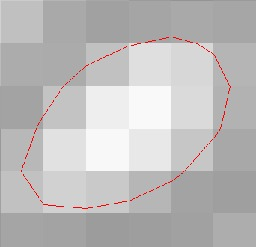
\includegraphics[width=\textwidth]{unmasked.jpg}
        \caption{Before Masking}
    \end{subfigure}
    ~ %add desired spacing between images, e. g. ~, \quad, \qquad, \hfill etc. 
      %(or a blank line to force the subfigure onto a new line)
    \begin{subfigure}[b]{0.15\textwidth}
        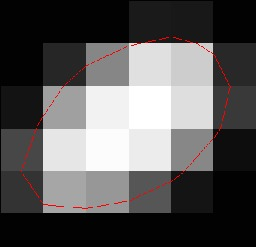
\includegraphics[width=\textwidth]{soft_masking.jpg}
        \caption{Soft Masking}
    \end{subfigure}
    ~ %add desired spacing between images, e. g. ~, \quad, \qquad, \hfill etc. 
    %(or a blank line to force the subfigure onto a new line)
    \begin{subfigure}[b]{0.15\textwidth}
        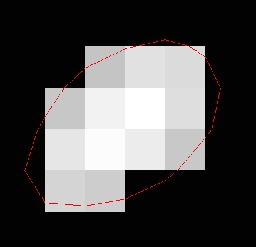
\includegraphics[width=\textwidth]{hard_masking.jpg}
        \caption{Hard Masking}
    \end{subfigure}
    \caption{An example of a masking operation}\label{fig:animals}
\end{figure}

\noindent
Figure 1 demonstrates an example use of a masking operation \cite{2:online}.
In this project, the operation will be used to remove irrelevant information (i.e. anything that isn't the robotic hand). 

\subsection{Design Rationale}
Clearly, this project is beyond our expected level of knowledge.
With this in mind, it is clear that opting for tools that can be tried quickly and repeatedly is critical to a successful end product.
It is possible that we'll change our planned implementation along the way and will require the reworking of fundamental steps along our path.
With the tools that have been designated, sudden changes will not be catastrophic to the project.

\subsection{Conclusion}
Upon project completion, the computer will be able to identify the robot arm in real time.
At least one of the methods used will beat the straw man approach of k-mean clustering without applying nearest neighbor.
Ideally, the computer will be able to correctly identify about 90\% of the pixels shown as either part of the arm or not in real time.
Specifically, the 90\% metric should apply to the region of an image with the arm in it, defined as the smallest rectangle in the image that includes the entirety of the arm.
However, if this arbitrary metric is not achieved, it will show that this approach will not generally be successful and an alternate approach (being developed by another person) will be used instead.
If this method proves successful before the deadline, there are also some stretch goals for the project, such as performing similar methods with objects for the robot to pick up.
Another stretch goal is to ensure that both methods can run simultaneously in real time.


\newpage
\section{Connor Campbell's Tech Review}
Note: Due to merging issues, references in this document only refer to its original References

\subsection{Introduction}
This project involves teaching a computer to grab objects with a robotic hand. To do this, the computer must
have an adequate understanding of the environment. The computer will be trained to identify objects through
computer vision and machine learning using a neural network. However, there are many different kinds of
neural networks and a few different ways to train them.

\subsection{Neural Network Structure}
There are many types of neural networks that are good at fulfilling different jobs. Three particularly common
ones include Feed Forward, Recurrent, and Convolutional.

\subsubsection{Feed Forward Neural Networks}
Feed Forward is perhaps the most generic of neural networks [1]. Feed Forward neural networks consist of
three parts: the input layer, the optional hidden layer (or layers), and the output layer. Each layer consists of
several neurons, which take in values from the previous layer, multiplies them by weights, then outputs the
value to all neurons on the next layer, usually after applying a function that maps the result to a certain range
[1]. The input layer is the exception, as it simply provides the input values to the first hidden layer.
Most neural networks (and all of the ones discussed in this review) follow the same basic structure, with
different types implementing additional features, such as memory. The advantage of Feed Forward networks
is their simplicity. If a given problem can be solved by a Feed Forward network, it may be easier to implement
than other solutions.

\subsubsection{Recurrent Neural Networks}
The primary difference between Recurrent and Feed Forward networks is that the neurons in the hidden layers
of an recurrent neural networks receive their own output as input in the next iteration [1]. This gives the
network a sense of memory, which gives them an advantage in problems where the program needs to make
several related decisions. If the best output for a given input depends on either the previous input or output, a
recurrent neural network is probably worth considering.

\subsubsection{Convolutional Neural Networks}
Convolutional neural networks are frequently used in computer vision [1]. Due to the sizes of images, fully
connected networks (in which each neuron takes input from all of the neurons in the previous layer) may
require far too many calculations [2]. To alleviate this problem, convolutional neural networks use specialized
neuron layers called convolutional layers and Pooling Layers.

While most layers in neural networks are fully connected, convolutional layers are not [2]. Each neuron
only looks at a specific range within the image, and several neurons are connected to that range, looking for
different patterns [2]. Pooling Layers are used to reduce the data being worked on between convolutional layers
by removing unnecessary information [2]. These specialized layers allow the network to examine large input
fields (such as the color values for the pixels in a large image) without overworking.

\subsection{Network Training}
An important detail in neural networks is the weights neurons use in calculations. These determine how the
program processes the inputs into the outputs. These values can not be reasonably determined by a human, as
there are too many interconnected parts. As such, they are initially chosen at random and then adjusted through
a training process, which can be done in a variety of ways.

\subsubsection{Back Propagation}
Back propagation is the most common form of training for neural networks. First, the network is given an input
for which the desired output is known. The network calculates an output with its current weights and that
output is compared to the desired one to determine the error [3]. Based on the output of the previous layer, the
weights are adjusted so that the output becomes closer to the desired output. Finally, an error for the previous
layer is determined based on the output layer's error and the new weights, and the process is repeated for that
layer [3]. Hence the name "back propagation" comes from stepping backwards through the network.

This algorithm is especially efficient since it can be done through matrix operations. The layers of a network
can be modelled as a series of matrices that are multiplied to an input vector. Back propagation can be performed
in a similar manner.

\subsubsection{Genetic Algorithm}
Neural networks can also be trained using genetic algorithms. Genetic algorithms mimic natural selection
by generating a population of solutions at random, eliminating less successful solutions, and reproducing
successful ones with slight alterations. Over time, the solutions become better and better.

Genetic algorithms have an advantage in situations where the exact desired output for a given input is
unknown. For instance, consider a neural network being trained to play a game or otherwise compete against
a human or other program. It may not be possible to judge each decision or move that it makes in any
scenario, making back propagation impractical. However, the fitness of the network can be directly measured
and compared to others based on its win rate.

Another major advantage to the genetic algorithm is that both the weights and the structure of the network
can be learned. With back propagation, the number of hidden layers and the number of neurons per layer are
predetermined by the programmer, but it can be rather arbitrary what structure is best for a given problem.
Genetic algorithms can adjust the structure as well as the weights, potentially making better decisions than the
programmer.

Genetic algorithms have some disadvantages. They effectively train a large number of neural networks at a
time, requiring much more memory and computing power.

\subsection{Conclusion}
Since this project involves computer vision, and convolusional networks are specifically designed for that, our
solution should probably incorporate something similar to that. It may be useful for the computer to take
previous input into consideration over time, which would encourage the use of recurrent neurons in the feed
forward layers. However, our program will already have access to the information that would provide.

For this project, the desired outputs can be known, so the genetic algorithm would be a poor choice.

\subsection{References}
[1]	K. Maladkar, 6 Types of Artificial Neural Networks Currently Being Used in ML, Analytics India Magazine, 31-Aug-2018.
[Online]. Available: https://www.analyticsindiamag.com/6-types-of-artificial-neural-networks-currently-being-used-in-todaystechnology/.
[Accessed: 01-Nov-2018].

\noindent
[2]	A. Karpathy, Convolutional Neural Networks (CNNs / ConvNets), in CS231n Convolutional Neural Networks for Visual Recognition.

\noindent
[3]	Nielsen and M. A., Neural Networks and Deep Learning, Neural networks and deep learning, 02-Oct-2018. [Online]. Available:
http://neuralnetworksanddeeplearning.com/chap2.html. [Accessed: 01-Nov-2018].



\newpage
\section{Chase McWhirt's Tech Review}
Note: Due to merging issues, references in this document only refer to its original References
\begin{abstract}
In this technology review, three technical ideas for the robotic grasping will be considered with three different technologies or plans of implementation each.
The three ideas that will be considered are data collection, qualifying data, and analyzing data (specifically, neural network frameworks geared towards analyzing data).
Each topic will have a suggestion that will be used to direct the group's plan for implementation.
\end{abstract}

\subsection{Introduction}
The robotic hand grasping project that my group will be accomplishing is a specific piece within a larger project.
Really, robotic hand grasping encompasses the goal behind the larger project.
In general, robotic hands are one of the most difficult limbs to develop.
In the larger scope of this project, our robotic hand has no sense of touch (tactile sense in and of itself is difficult to develop and work with) and can only have visual awareness of a scene.
The goal for the larger project is to be able to put the robot arm in a box and be able to run many real world simulations from any external location.

With context out of the way, it will be a lot more clear how we're constructing our piece of the project.
Our piece is going to cover lighting issues primarily.
Our focus will be for the robot arm to maintain complete awareness over its location (particularly when it casts a shadow over itself).
It may seem like it should a straight forward process if we understand the robot hand's physical specifications.
However, when the robotic hand begins approaching the object, obfuscation and lightning can completely ruin the computer's vision of a scene.

\subsection{Technology Overview}
After talking with our sponsor, we've developed a plan that will incorporate some technologies.
I will talk about these options first, then explore two alternative options.
In order to speak on these technologies, it's important to understand our planned solution at a high level.
We'll be taking video footage and / or pictures of the robot arm.
This media will cover various angles and lighting situations.
We will then define where the arm is in any given frame or picture.
We will feed this into a machine learning algorithm in hopes of generalizing our data.
After learning, it should be able to successfully identify the arm's location with 95\% accuracy instead of the current 85\% accuracy.
Depending on how easily we can accomplish this, we've set a stretch of goal of doing the same thing with the object the hand will grab.
If we complete that stretch goal, we'll do both at the same time as our final stretch goal.

\subsection{Step 1: Data Collection}
In this section, I will cover how exactly we intend to collect information.
There's a few simple ideas that come to mind.
First, we could follow the route of a digital camera for filming or to manually take pictures.
Second, we could circumvent the vision issue by creating a physically accurate, three dimensional simulation.
Lastly, we could also find images, videos online or create simulate videos to mimic training data.
To clarify the distinction, in the second idea, the AI would have to not need an impression of reality.
In the third idea, the AI could use artist renditions of reality to better understand literal reality.

\subsubsection{Image Feed}
Whether it's through video or taking a bunch of pictures, this in and of itself is pretty straight forward and easy.
However, the data itself is harder to work with later on. Can we really objectively define what is and isn't mostly an object pixel?
The video stream the machine learning will be applied on will be pretty low resolution in comparison to potentially 4K photographs or video feed.
Though higher resolution images might help our neural network with accurately labeled objects, it's possible the machine learning process could be slowed down via more data input than is necessary.

\subsubsection{Pure Simulation}
Though I thought of this idea early on, it should be noted that our sponsor has advised against it from the start.
This is due to a competing implementation being completed by another team that is doing it this way.
The idea behind this would be to maintain a constant, accurate, and complete three dimensional understanding of a scene.
Using the Unity Engine, you could have a simple program that stores the position of the artificial objects corresponding to real world objects.
The downside is the difficulty and tedium of creating these assets and handling them.
There's also the problem that this method is fairly computationally expensive versus running a machine learning algorithm.

\subsubsection{Outsourcing}
Outsourcing can mean two things in this instance.
First, we can gather images of objects similar to ones the hand might hold.
Training our algorithm with this could potentially give it the widest scope of objects it could work it.
However, a major challenge would to minimize the randomness manually by finding high quality images that are similar (perhaps the same object at a different angle).
Alternatively, we can use Blender or Unity to create artistic renditions of an object (like a ball or a cube) and create a video of a light circling an object.
We can also artificially cast shadows with this method as well by creating duplicate objects.
The downside to this approach would be that our algorithm would be trained on data that could potentially be far different from real world objects we'll be using.

\subsubsection{Suggestion}
Of the three, creating an image feed ourselves with the objects we'll actually be attempting to manipulate seems like the best option.
It has the advantage of letting us make the images at the right resolution (which might be closer to our AI's camera resolution than purely higher resolution), use a neural network for lower memory overhead, and will be the easiest to produce and try.
There were no research metrics here because I didn't think there would anything for a concept like this.
It's mostly speculation anyways that can only be resolved by trial and error.


\subsection{Step 2: Qualifying Data}
Basically, how do we interpret the reality of the data we're seeing.
How do we define pixels that are a part of the object and those that aren't.
This will involve feeding images we generate into an image editor that can easily label photographed objects accurately.
First, Photoshop comes to mind first as it has a labeling feature included.
Secondly, After Effects should be considered as it detect objects within video feed.
Finally, Gimp should be considered as a free alternative.

\subsubsection{Adobe Photoshop}
This is what is advised by our sponsor. It has functionality that can trace objects [1].
A potential downside is having to also use Photoshop meta data in order to train our neural network.
Though, this downside, is present in both alternatives.

\subsubsection{Adobe After EFfects}
Our TA suggested Adobe After Effects for it's ability to label objects within video feed [2].
In the video editing process, it's possible to label objects from its background.
This is the effect seen after filming something with a green screen background.
After Effects has a major downside of costing money and not being available to students.

\subsubsection{Gimp}
Finally, GIMP was a suggestion made by McGrath.
It has the major benefit of being free software, which would allow us to access the capability of object labeling much more easily.
It has the downside of not being preferred by our sponsor.

\subsubsection{Suggestion}
Gimp seems like the best option objectively.
It has the same capability of Photoshop to label images and layer them.
It maintains an edge by free and open source unlike Photoshop.


\subsection{Step 3: Analyzing Data: Neural Network APIs}
Finally, probably the most interesting part of the project to me, the machine learning algorithm that would handle our data.
In this section, I'll purely be looking at neural network APIs.
I'll be ignoring the fault of neural networks (which appears to primarily be their random effectiveness and failure to generalize effectively). 

\subsubsection{TensorFlow}
This is Google's open source neural network API.
One partial downside is that its a relatively young library, it makes up for this by having thousands of contributors which is at least twice as much as all other neural network APIs [4].
Another critical downside is that its not as fast as other libraries [5].

\subsubsection{Theano}
This is a very flexible neural network library.
It also has the benefit of age and having lots of documentation [5].
"Theano allows you to define, optimize, and evaluate mathematical expressions involving multi-dimensional arrays efficiently" [4].
Many major neural network libraries build on top of Theano, which could be beneficial in narrowing the scope towards our project.

\subsubsection{Caffe}
"This library is specially optimized for vision tasks... it is often among the fastest libraries when benchmarked on vision tests" [5].
This library seems like it's well suited to the type of project we're trying to complete.
Since it's also very fast, it has the benefit of being test friendly.
This means, we can take multiple data approaches without the need to push back deadlines.

\subsubsection{Suggestion}
It's difficult to make a suggestion here.
Though TensorFlow and Theano have the benefit of being popular and flexible, I believe Caffe would be the best choice.
It's experimentation friendly. It's also designed to handle images, which could be exactly the kind of API we need.


\subsection{Conclusion}
While it's difficult to find the best approach with no experience, research has led me to believe that taking pictures of images ourselves, using GIMP to label them, and then train a neural network via the Caffe library seems like the best first approach.
The primary benefit of this combination is that it's easy to test freely.
It'll also begin working very quickly, which is good for only a three month deadline.
We can always switch out pieces as we quickly find they're not quite as good as expected with little blow back in terms of time consumption.
Thus, I my overall suggestion is to take pictures ourselves, process them with GIMP, and train a neural network via Caffe.

\subsection{References}
[1]	https://www.adobe.com/products/photoshop.html

\noindent
[2]	https://www.adobe.com/products/aftereffects.html

\noindent
[3]	https://www.gimp.org/

\noindent
[4]	https://www.kdnuggets.com/2018/04/top-16-open-source-deep-learning-libraries.html

\noindent
[5]	https://www.quora.com/What-is-the-best-open-source-neural-network-library

\newpage
\section{Jiawei Mo's Tech Review}

\subsection{Introduction}
My role of this project is to build up the graphic scene and deal with adjusting lighting changes of the object. It is a repeatable process since the machine learning algorithm will store precise data and drop lower reliable cases. Then, it will circle the processes to improve the accuracy of stored image data. 

\subsection{Target}
Unlike humans, robots do not have a sense of touch, and rely on cameras for vision. As such, computer vision is an important part of designing robots to interact with the world on their own. Our task is part of an ongoing project attempting to improve a computers understanding of a three dimensional environment through machine learning and computer vision; developing computer algorithms to help robotic arms determine the appropriate path to grasp an object. At the moment, the computer is using two stationary cameras placed at different angles facing the arm and the object, and analyzing their feedback to determine the objects position and type. \\

\noindent
The current setup has a few problems. To begin with, lighting changes can make it difficult to identify an object. When the hand is covering the object, the shadow changes the light captured by cameras. Also, if the environments light intensity changes, it will result in a color change to captured streams. The computer is expecting pixels representing the object to be in a certain range in the RGB spectrum, and such changes will potentially move the apparent colors out of the expected range. As a result, the computer fails to recognize the presence of the object its looking for. We could expand the expected color range, but that could cause the computer to recognize parts of the image that are not the object, such as the background, as part of the object. Our goal is for the computer to recognize the object in different levels of light, without that issue. \\

\noindent
Another problem is when the robotic hand gets in the way of the cameras. Since the cameras are at fixed positions, the robotic arm will block parts of the object when it moves in to pick it up. As a result, the apparent shape of the object on the screen will change, causing the computer to fail at identifying it and cannot accurately determine its position and shape. \\

\noindent
The end goal of this project is to create a software that will accurately identify a robotic arm in a given image. Several possible solution plans have been created with the help of the client. The client is going to take many photos (as HSV image type) of the robotic arm and supply a mathematical description of the arm's pose for each photo. Next, a straw man solution will be generated by running a k-means clustering method on all of the images, which will yield a naive method for identifying parts of the robotic arm. This will act as a base line: the other solutions will be considered successful if the prove to be better than the straw man solution.

\subsection{Detailed Pieces}
This section will demonstrate three key pieces of the project and brainstorm other optional technologies that can solve the same problem.

\begin{enumerate}
\item Capture of the Data
    \begin{enumerate}
    \item Goal: \\
    In order to track the robotics grasping pose, it requires that the computer is supposed to compare the monitored streams from cameras with stored data in the memory. Thus, previous task is to capture objects' data by taking images from various viewpoints to build three dimension scene. The followings are three methods to handle this issue.
    \item Image Sets \\
    This technology is the method to capture objects' data in this project. We intend to set up a box that keeps environmental light out. Then, taking pictures of the object under a certain light intensity in the box. This aims to keep recorded RGB values of each object the constant. Further, changing the viewpoint of the camera and repeating image capturing. Finally, all objects' 3D images will be stored in the computer. By this solution, we probably need to create over 150 sets of images of every single object to support sufficient sources for the computer to form detailed 3D scene of the object. Also, we need to be very careful to deal with lighting. Since this step is to create objects' data on the computer, there is no doubt that data is not allowed to contain wrong information. Notice that the surface color is one of the information that the computer is going to use to distinguish the type of objects. Moreover, colors are represented by RGB values. Each of three primary color has a value interval from 0 to 255, if the computer treats it as an integer. Even though red 250 and red 200 both present red color to the object's surface, the computer will not put them into a single category. Therefore, it is necessary to create images with precise and constant lighting, which lead to a constant surface color. 
    \item 3D Printing \\
    Another approach that comes out from my mind is 3D printing. The previous point is to capture objects' data. Nevertheless, this method is to construct 3D models with computers. In this case, the objects' data is in the memory at the beginning. There is no need to worry about transferring physical objects' specifics into data. A 3D printer can carve objects with precise information given by the computer \cite{101:online}. Then, using created objects to test algorithm of grasping pose tracking. There might be a concern that how accurate a 3D printed object will be. Compared to original object that is built in computer, a physical object may have flaws. Therefore, this option has additional requirement, which is to measure the specifics of each object. For instance, it is obligatory to measure the length of each edge of the polygon, referring to a cube. Developers might define required accuracy to be 0.01 centimeter and abandon objects not within the range. 
    \item Panorama \\
    Back to capture images, a better camera or more powerful device can help us to obtain physical objects' data. Panoramic camera shows a possibility to create 3D scene of objects through 360 degree panorama \cite{102:online}. This solution cost much more than the first option since a powerful panoramic camera is expensive. However, it does save lots of time to photograph hundreds of object images. Similarly, it needs to interact with lighting set. As mentioned previously, we need to keep objects' surface colors to be constant variables. 
    \item Comparison \\
    To highlight, the images sets is the cheapest and simplest solution to handle data collection. Either 3D Printing or Panorama will cost much more than images sets. 3D Printing requires a long time to build up the sophisticated models and checks. Moreover, it asks for material sources to print out models. Similarly, Panorama equipment is expensive for this project and accurate data capturing costs a lot more. 
    \end{enumerate}
\item Color Changing
    \begin{enumerate}
    \item Reminding \\
    To begin with, lighting changes can make it difficult to identify an object. When the hand is covering the object, the shadow changes the light captured by cameras. Also, if the environmental light intensity changes, it will result in a color change to captured streams. The computer is expecting pixels representing the object to be in a certain range in the RGB spectrum, and such changes will potentially move the apparent colors out of the expected range. 
    \item Neural Network \\
    Our completed project will be using neural networks. Overall, we'll be using a supervised learning approach. Caffe is a robust, flexible framework that works well for this project in many ways \cite{103:online}. It's easy to work with, works efficiently, and is tailored for many project specifications. This framework is classified as a deep learning framework. For proper implementation, three deep learning principles should be considered. Deep learning uses a cascade of multiple layers of nonlinear processing units for feature extraction and transformation. As a project specification, implementation will follow supervised learning. Finally, the neural networks will learn multiple levels of representation that correspond to different levels of abstraction; the levels form a hierarchy of concepts \cite{deep_learning}.
    \item Color Sensor \\
    This option is using the color sensor to detect the object surface color. The color sensor is a device that can compare objects' colors with previously referenced colors to improve color detection \cite{104:online}. Once two types of colors are within a certain acceptable range of error, the sensor will output the results. With various referenced labels, even though the background has a subtle difference in color, the sensor could detect it in a fast speed. There are other advantages, including automatically adapting to wavelengths, detection of tiny difference in gray value and independence of the color of the label and the background. This option could replace the function that is dealing with colors. 
    \item Gray Scale \\
    Since working on color is a tough task, there is a method to only compare two images' gray levels \cite{105:online}. This option allows us to avoid complex computation of colors, including discrete algorithm. The gray scale is a single value that is represented on a single channel. To demonstrate, the image will be totally black while its gray level is 0 and white for maximum gray value. The first option utilizes diffuse and specular to calculate the objects' surface colors in order to restore the colors variables in computer for comparing with referenced data. In this option, the brightness of objects will be used to compare because more bright the object is, a higher gray value it will show. 
    \end{enumerate}
\item Pose Tracking
    \begin{enumerate}
    \item The Aim \\
    The purpose of the project, 3D object pose tracking for Robotics Grasping, is to successfully track the hand and object position. It is improved by dealing with lighting changes and shades. 
    \item Tracking System \\
    The object tracking system currently used by the University's robotics team is to use cameras placed aside the object to produce video streams to a computer. By analyzing frames of certain images, the computer will label each pixel of each image with terms of background, object and robotic hand, which is the way for computer to distinguish the object and then track the pose of robotics grasping. Currently, it accounts for this by identifying a large range of colors as potentially being part of the object. This, of course, results in a lot of false positives (pixels being labeled as part of the object when they actually aren't). An advanced approach will allow the computer to adjust the expected average for the specific lighting with a smaller acceptable range. 
    \item Motion Capture \\
    This option, indeed, will cost a lot more than our current tracking system. However, this technology afford more precise position tracking of various objects, even human action. Some companies, including Sega Interactive, have launched a variety of commercial motion capture devices. A tracker is set at a key part of the moving object, and the position of the tracker is captured by the motion capture system. Then, a computer processes obtained data to generate the three-dimensional space. This technology is widely used in movie and game field to capture human actions \cite{106:online}. One sensor is called inertial navigation sensor, which measures the characteristics of the athlete's motion acceleration, azimuth, and tilt angle. This approach is not effected by environmental disturbances and blocks. The capture accuracy is extremely high and the sampling speed could reach 1000 times per second or higher. 
    \item OpenCV \\
    It is an open source computer vision library \cite{107:online}. OpenCV is written by C++ and its main interface is also C++, but still retains a large number of C language interfaces. The library also has a number of interfaces to Python, Java, MATLAB/OCTAVE (version 2.5), C\#, Ruby and GO. OpenCV program is fast, stable and strongly compatible. It is a choice to get rid of some special solutions that rely on hardware, such as video surveillance, manufacturing control systems, medical equipment. OpenCV focuses on real-world and real-time applications, and its execution speed is greatly improved by the optimization of C language. Fields, like human computer interaction, action recognition and robotics, are gaining benefits from this technology. We can implement our OpenCV program to track object position. 
    \item Comparison \\
    Without doubts, the project is going to use its own system since this project belongs to a huge project. Therefore, the data shifting between different teams can not have conflicts. On the contrary, other technologies are considered while the current solution fails to implement or has troubles to produce reasonable outcomes that reveal the solution is incorrect partially or having bugs. 
    \end{enumerate}
\end{enumerate}

\subsection{Conclusion}
This essay reviews three technologies that are used in the project and introduces other implementable solutions. A comparison of each section gives the reason why the technology is chosen and whether another technology can replace it. 


\newpage
\section{Weekly Blog}
%---------all team members' posts \\
%formatted nicely and clearly distinct from one another \\
%include all members posts, clearly distinct, clearly organized \\
%scrub blog posts of information you don't want others to read \\

\subsection{2018 Fall}
\begin{center}
\begin{tabular}{|p{0.3\linewidth}|p{0.3\linewidth}|p{0.3\linewidth}|}
\hline
\multicolumn{3}{|c|}{\textbf{2018 Fall: Week 3}} \\
\hline
\textbf{Connor Campbell} & \textbf{Chase McWhirt} & \textbf{Jiawei Mo} \\ [0.5ex]
\hline\hline


&
\textbf{Progress:} Managed to contact my assigned TA, my group sponsor, and my other group members.
Finished a rough draft of my problem statement Thursday before I had made contact.

\textbf{Problems:} Still need to meet with everyone and have a discuss the project in more depth.
Didn't really base my problem statement on anything other than the project description(s).

\textbf{Plans:} I am going to try and meet with everyone Monday, that seems like the day we're leaning towards.
I also want to clarify the project so I can make a better, more official, problem statement.
&

\\ \hline
\end{tabular}
\end{center}

\begin{center}
\begin{tabular}{|p{0.3\linewidth}|p{0.3\linewidth}|p{0.3\linewidth}|}
\hline
\multicolumn{3}{|c|}{\textbf{2018 Fall: Week 4}} \\
\hline
\textbf{Connor Campbell} & \textbf{Chase McWhirt} & \textbf{Jiawei Mo} \\ [0.5ex]
\hline\hline

Last week, due to communication problems, we weren't even able to properly meet , and only did individual drafts for the problem statement. This week, we all properly met each other, and two of us met with our client and got a clearer picture of the project. We also completed the problem statement together. I'm unsure of our specific team plans, but we plan on meeting with our client again soon to iron out a few details that we are unclear on.
&
\textbf{Progress:} We got a group problem statement out.
We met up and had a few good discussions about the problem statement.
However, this has only revealed some underlying problems.

\textbf{Problems:} Our Problem Statement is still in a rough draft state, essentially.
We realized we don't have a good enough understanding of the solution to the two problems we're hoping to solve.
This lack of a good understanding has led us have metrics that will probably be inaccurate later on development.
I'm not sure if there's a solution to finalizing our problem statement.
We turned in what we could.

\textbf{Plans:} We definitely need to meet with our project sponsor again to iron out the solutions and the metrics we're using to verify our solutions.
We may even need to redefine the problem because it has become increasingly unclear.
I'm not sure what's in store next for this class, but for the project, we need to have a more thorough discussion with our project sponsor as soon as possible.
&
Our group has had a meeting with client on Wednesday. We talk about project requirements and basic information that we need. Group has not seen our TA and talked to him since he has to attend a presentation. Also, we have not confirmed a stationary schedule for communicating every week. We plan to finish our problem statement due by Friday with details of our project and prepare a new schedule for future meetings.
\\ \hline
\end{tabular}
\end{center}

\begin{center}
\begin{tabular}{|p{0.3\linewidth}|p{0.3\linewidth}|p{0.3\linewidth}|}
\hline
\multicolumn{3}{|c|}{\textbf{2018 Fall: Week 5}} \\
\hline
\textbf{Connor Campbell} & \textbf{Chase McWhirt} & \textbf{Jiawei Mo} \\ [0.5ex]
\hline\hline

Forgot to write a blog post this week.
&
\textbf{Progress:} No real progress to report.
We have a Github repository for when we start coding and everyone is a part of it.
Connor managed to meet with our sponsor, Cindy, on Thursday.
I completely forgot to check my email and it didn't hit me until a couple hours ago that I should have kept an eye on that and met as well.

\textbf{Problems:} Meeting with our sponsor is difficult so far.
It might be better if we make someone the note taker.
Then we can have that person meet with her as needed.

\textbf{Plans:} I'm going to try and get into contact with the group and decide a plan for completely the requirements document.
I'm also going to talk with them and see if we can get a note taker.
I'd be willing to do it myself but maybe we can rotate the responsibility.
&
Communicating with client to understand requirements. I have to learn about OpenRave that can generate normal vector for each polygon's surface. This allows to use the nomal vectors to deal with lighting reflection. With knowing functionality of OpenRave, I could start to design our project solution. I plan to follow some tutorials of OpenRave next week. 
\\ \hline
\end{tabular}
\end{center}

\begin{center}
\begin{tabular}{|p{0.3\linewidth}|p{0.3\linewidth}|p{0.3\linewidth}|}
\hline
\multicolumn{3}{|c|}{\textbf{2018 Fall: Week 6}} \\
\hline
\textbf{Connor Campbell} & \textbf{Chase McWhirt} & \textbf{Jiawei Mo} \\ [0.5ex]
\hline\hline

We've completed draft 1 of the requirements document. Our client is on vacation this weekend and said she won't respond to emails until she's back, so we'll likely ask her to look it over next week. I completely forgot about the tech review rough draft, which was entirely my fault, but I'll try to at least have something by the time we do in-class review.
&
\textbf{Progress:} We managed to get in the rough draft for the requirements document and I'm going to get in the tech review.
I also managed to get to meet the TA, which feels like good progress.
Oh, we also made some rules about how to meet as a group.

\textbf{Problems:} I just remembered, we were going to set up Slack in after class on Thursday but I didn't go to class then.
Also, my tech review rough draft is probably going to be a little empty.
Hopefully feedback will contain ideas for how to fill those gaps because I couldn't really imagine how to break up our project into three parts.

\textbf{Plans:} I'll organize everything we need to get Slack up over the weekend.
That was my mistake.
It shouldn't be too difficult and then we can review and see if there was anything else we were going to do...
I think we were going to put our .tex documents on Github as well.
&
Starting reading document and learning some program tools that might be used in this project. There are too many writings so that I don't have enough time to focus on graphics part, which is a problem. I plan to keep researching and trying some sample codes.
\\ \hline
\end{tabular}
\end{center}

\begin{center}
\begin{tabular}{|p{0.3\linewidth}|p{0.3\linewidth}|p{0.3\linewidth}|}
\hline
\multicolumn{3}{|c|}{\textbf{2018 Fall: Week 7}} \\
\hline
\textbf{Connor Campbell} & \textbf{Chase McWhirt} & \textbf{Jiawei Mo} \\ [0.5ex]
\hline\hline

This week we worked on our tech reviews and set up a Slack channel for more convenient communications. We didn't communicate much in making sure our topics didn't overlap, but it didn't turn out to be a problem. We should probably meet with our client again soon.
&
\textbf{Progress:} I got the rough draft in for the individual tech review done.
I think I should be able to incorporate the suggestions, research, and meet the word count by midnight.

\textbf{Problems:} There was concern with crossover on the tech review since there are three main subject matters we've discussed with our sponsor.

\textbf{Plans:} I'm going to fill in the gaps in my research for the paper and proceed with the areas of interest I was already covering.
The chance this will require us to research more later isn't too high so I think I'm happy with that outcome.
&
Finished tech review. Knowing that there are various methods to solve our project problem. I keep learning about the technology that we are going to use and being familiar with it. Also, I focus on details that client gave us to think about effective solution.
\\ \hline
\end{tabular}
\end{center}

\begin{center}
\begin{tabular}{|p{0.3\linewidth}|p{0.3\linewidth}|p{0.3\linewidth}|}
\hline
\multicolumn{3}{|c|}{\textbf{2018 Fall: Week 8}} \\
\hline
\textbf{Connor Campbell} & \textbf{Chase McWhirt} & \textbf{Jiawei Mo} \\ [0.5ex]
\hline\hline

We didn't really do much this week, though we are planning to meet with our client again soon.
&
\textbf{Progress:} There wasn't any progress made this week.
Though, from my last post, I got a my tech review final solo draft done.
Maybe it would be a good idea to share with the group.
Though, maybe it's better to wait until the group version needs to be worked on.

\textbf{Problems:} I heard the grading might be arbitrarily strict.
I haven't gotten my grade for it, but I did reach the word count and feel confident enough about it.
It did pass the originality report which is good.
I also missed a meeting with the TA this week.
I completely blanked it.
It's been a little hectic this week.

\textbf{Plans:} I don't really have any plans.
We've talked about possibly meeting with our sponsor again and sharing our progress with them, but I don't think anyone else has made arrangements yet.
I don't think it's necessary quite yet until our next group assignment.
&
Keeping doing researches and learning about new stuff. I try to determine a specific direction to start to work by reviewing online lectures, technique videos and tools implementation.
\\ \hline
\end{tabular}
\end{center}

\begin{center}
\begin{tabular}{|p{0.3\linewidth}|p{0.3\linewidth}|p{0.3\linewidth}|}
\hline
\multicolumn{3}{|c|}{\textbf{2018 Fall: Week 9}} \\
\hline
\textbf{Connor Campbell} & \textbf{Chase McWhirt} & \textbf{Jiawei Mo} \\ [0.5ex]
\hline\hline

Forgot to write a blog post this week.
&
\textbf{Progress:} Well, unfortunately, I can't say much progress was made.
We all successfully met with our TA and got some troubling news.
I suppose knowing there is a problem is progress, to some extent.

\textbf{Problems:} Apparently, based on the documentation we've written so far, we are not prepared for completing the project.
I admit, my own understand is limited.
The scope of the project makes sense and seems doable... 
Until we start considering implementing machine learning on our data in any capacity.
The intention for joining this project was to learn about machine learning and implement it in some way to a project.
However, we have not been given a direction to look and haven't done independent research either.

\textbf{Plans:} Our plans are to keep doing the documentation as best as we can, meet with Kirsten, and meet with our sponsor, Cindy.
I would like to have a crystal clear understanding of the project for myself so I know how to fulfill any of the requirements.
&
Starting learning OpenCV functionality, including basic rules, syntax, matrix computation, and so on. One obstacle is the lack of machine learning experience. Project problem situation is understandable but I need to research on machine learning models and learn how to implement it. Our group plan to meet the client to ask about specific machine learning materials we need.
\\ \hline
\end{tabular}
\end{center}

\subsection{2019 Winter}
\begin{center}
\begin{tabular}{|p{0.3\linewidth}|p{0.3\linewidth}|p{0.3\linewidth}|}
\hline
\multicolumn{3}{|c|}{\textbf{2019 Winter: Week 1}} \\
\hline
\textbf{Connor Campbell} & \textbf{Chase McWhirt} & \textbf{Jiawei Mo} \\ [0.5ex]
\hline\hline
\textbf{Progress:} Nothing really happened this week. We were getting settled back in after the break.

\textbf{Problems:} Data set hasn't been received yet.

\textbf{Plans:} Set up weekly meetings with our client.
&
\textbf{Progress:} None, unfortunately.

\textbf{Problems:} Week 1 was extremely hectic for me.
I got my PIN later than expected and had to register during week 1 because of that.
The fact we included working in week 1 in our plans has backfired a little but I'm sure we can make up for it.

\textbf{Plans:} We've arranged times to meet consistently with our sponsor and our TA.
It'll be greatly beneficial to meet with them every week.
I also decided to go half time this term so I can make sure the project is good.
&
Our group contacts with our client and prepare a meeting to talk about project beginning. We plan to have a meeting in the next week then we could be hands on the project. 
\\ \hline
\end{tabular}
\end{center}

\begin{center}
\begin{tabular}{|p{0.3\linewidth}|p{0.3\linewidth}|p{0.3\linewidth}|}
\hline
\multicolumn{3}{|c|}{\textbf{2019 Winter: Week 2}} \\
\hline
\textbf{Connor Campbell} & \textbf{Chase McWhirt} & \textbf{Jiawei Mo} \\ [0.5ex]
\hline\hline

\textbf{Progress:} We've set up weekly meetings with our client

\textbf{Problems:} We have yet to receive the data set

\textbf{Plans:} We can't really do much without the data set
&
\textbf{Progress:} We met with both TA and our sponsor for the first time this winter.
It was felt like good progress overall until we found out about the problems.

\textbf{Problems:} We don't actually have the data set yet.
I had assumed (because we were told) that the data was already collected during finals week/winter break.
In a way, I'm relieved because week 1 was a mess but I'm also suddenly extremely concerned because there's nothing to do yet.
Fortunately, we're getting the data Thursday... Hopefully...

\textbf{Plans:} We'll work on the poster and the elevator pitch over the weekend when we're all free.
At least that will feel like minor progress.
&
Group has met with our TA and client. We are told that they are still preparing on data and we have to wait. Another group might collect a part of the data right now. To label data will cost a number of hours, that is our concern.
\\ \hline
\end{tabular}
\end{center}

\begin{center}
\begin{tabular}{|p{0.3\linewidth}|p{0.3\linewidth}|p{0.3\linewidth}|}
\hline
\multicolumn{3}{|c|}{\textbf{2019 Winter: Week 3}} \\
\hline
\textbf{Connor Campbell} & \textbf{Chase McWhirt} & \textbf{Jiawei Mo} \\ [0.5ex]
\hline\hline

Our team is in an awkward position where we need data from our client before we can really do anything productive, and we've been waiting for that data for over a week. Apparently, when they were getting a data, they realized that their measurements were off and had to start over. If this goes on too long, maybe we should get some fake data just so we can practice the procedure for when we get the real data.
&
\textbf{Progress:} We met with our TA and sponsor again.
We finished the elevator pitch and poster and I've reframed the elevator pitch to be more goal oriented versus process oriented.
It feels a lot better and I feel pretty confident about EXPO, other than completing the project.

\textbf{Problems:} We STILL don't have the data.
This extremely concerning but I'm still trying to believe there's a way to make up for the nearly 100 hours of lost time we were supposed to put in.
(I'm saying this in reference to each person putting in 3-4 hours of work per credit per week.)
We haven't even gotten sample data we were promised much earlier on (basically one picture of the arm to practice photoshop masking with).
Our class Tuesday of Week 4, Kirsten mentioned how this is like a mission critical serious issue and has dectupled my cortisol levels.

\textbf{Plans:} I'm not sure what can even be done at this point.
There's nothing we can do at the moment.
Pretty concerning.
I can't express in words the feelings I'm having.
&
Group meets with TA to talk about our elevator speech and gets some advise. In addition, we are still waiting for the data sets from our client. They have troubles on pre-dealing with data. Data sets should be available on Friday but not. I plan to build up a Kmeans model and train it with hand writing image sets to evaluate the model performance.
\\ \hline
\end{tabular}
\end{center}

\begin{center}
\begin{tabular}{|p{0.3\linewidth}|p{0.3\linewidth}|p{0.3\linewidth}|}
\hline
\multicolumn{3}{|c|}{\textbf{2019 Winter: Week 4}} \\
\hline
\textbf{Connor Campbell} & \textbf{Chase McWhirt} & \textbf{Jiawei Mo} \\ [0.5ex]
\hline\hline

We've received some of the data we needed and are beginning the process of qualifying it. We plan to have 21 images processed and ready to train the initial "straw-man" method soon. After that, we'll be able to get started on the larger parts of the project.
&
\textbf{Progress:} Unfortunately, still not a lot (for me) at the moment.
We've got the data we need to get started.
It's not really what we planned on but I suppose it will suffice for the project.
Connor has identified images that each of us (7 images each) will create a mask for.
(Note, this blog post was done late. We got the initial data during week 5.)
We also had a class where we got to practice the elevator pitch.
Jiawei also coordinated with group 51 who we'll be meeting with Wednesday at 7:15 PM.

\textbf{Problems:} Got to start catching up with the actual project.
Tomorrow is probably when I'll start doing a lot of work.
Not sure what else to say other than we're four weeks behind and that feels pretty terrible.

\textbf{Plans:} I'm going to start working tomorrow on processing the data.
I'll also investigate the timeline see how much works needs to be done for us to be caught up.
We're planning on meeting to talk about the poster (with Kirsten and group 51).
I think summarizes it for this week.
&
Arm image sets are available and we start to label. However, group is still waiting for arm position data. We plan to finish the first 20 images labeling and then we can use position data to adjust our training set.
\\ \hline
\end{tabular}
\end{center}

\begin{center}
\begin{tabular}{|p{0.3\linewidth}|p{0.3\linewidth}|p{0.3\linewidth}|}
\hline
\multicolumn{3}{|c|}{\textbf{2019 Winter: Week 5}} \\
\hline
\textbf{Connor Campbell} & \textbf{Chase McWhirt} & \textbf{Jiawei Mo} \\ [0.5ex]
\hline\hline

\textbf{Progress:} We've created masks for 21 images by hand to train the initial straw-man

\textbf{Problems:} We still don't have what we need to complete the other methods

\textbf{Plans:} Jiawei is working on the straw-man, and we'll be asking our client how to go from here regarding the other methods
&
\textbf{Progress:} Nothing significant.
We've begun processing the images.
We're each going to manually create a mask for seven images using Photoshop.
Connor has picked out the images. 
Jiawei is practicing K-means.

\textbf{Plans:} We'll process the images and do the straw man method.
Still waiting for this .csv with the arm poses that they said they have.
&
Group is starting labeling pictures but I am worried about the slow progress. I am ready for using Kmeans to process the image sets.
\\ \hline
\end{tabular}
\end{center}

\begin{center}
\begin{tabular}{|p{0.3\linewidth}|p{0.3\linewidth}|p{0.3\linewidth}|}
\hline
\multicolumn{3}{|c|}{\textbf{2019 Winter: Week 6}} \\
\hline
\textbf{Connor Campbell} & \textbf{Chase McWhirt} & \textbf{Jiawei Mo} \\ [0.5ex]
\hline\hline

\textbf{Progress:} We're almost done with the initial straw-man method

\textbf{Problems:} We still don't have all of the data we need

\textbf{Plans:} We're going to talk to our client to see if we can get the missing data soon
&
\textbf{Progress:} Unfortunately, less progress has been made than expected.
I'm still frustrated with our progress, but since it's out of control, dwelling on that isn't good for me or the group.
To ensure I've covered all progress, we merged all of our work on Github, which includes the K-means straw man and the manually created masks.

\textbf{Problems:} I'm not sure how our K-means straw man method works since we didn't work on it together.
It's also in Python, which is one of my weaker languages.
Even beyond that though, we need a .csv with our robot arm's poses in order to do nearest neighbor operations.
I've been feeling bad about progress and how this project was a lot less interesting than expected.

\textbf{Plans:} Going to get the alpha done by our Wednesday meeting.
Keep asking for the .csv.
Perhaps doing a convoluted neural network to create a mask as a straw man so I will at least get to experience that.
Might do the same for support vector machines.
&
Client is out of the town and we miss the meeting. I almost finish Kmeans model and plan to meet with client to show her some results and talk about model adjustment. 
\\ \hline
\end{tabular}
\end{center}

\begin{center}
\begin{tabular}{|p{0.3\linewidth}|p{0.3\linewidth}|p{0.3\linewidth}|}
\hline
\multicolumn{3}{|c|}{\textbf{2019 Winter: Week 7}} \\
\hline
\textbf{Connor Campbell} & \textbf{Chase McWhirt} & \textbf{Jiawei Mo} \\ [0.5ex]
\hline\hline

\textbf{Progress:} We've pretty much completed the initial strawman/control method

\textbf{Problems:} While it was expected, the strawman method is quite terrible at getting results.

\textbf{Plans:} Other than the rough draft of the progress report, we need to get started on the other methods
&
\textbf{Progress:} Jiawei and I have worked on the straw man code.
I'm trying to get it finished such that it will do a list of images instead of one per program run.
(I think I might be referring to my analysis script here...?
I did modify the K-means script to learn more about it but that work was scrapped).

\textbf{Problems:} We're all feeling discouraged about the project.
It's nice that we were able to talk about it together.
We still have to work on it though, in whatever way we can.

\textbf{Plans:} Now that we can actually work on stuff.
(To clarify, I believe it was this week we learned there is no .csv and there are no stereoscopic pairs of images.)
Going to start working on this more consistently.
Also going to do this blog much sooner in the week because I hate losing points arbitrarily.
&
I have improved the current Kmeans algorithms to create masks for images but the areas out of the base show a lot of noises. I am waiting for client's reply and opinion. I am also looking for some solution to refine the outcomes.
\\ \hline
\end{tabular}
\end{center}

\begin{center}
\begin{tabular}{|p{0.3\linewidth}|p{0.3\linewidth}|p{0.3\linewidth}|}
\hline
\multicolumn{3}{|c|}{\textbf{2019 Winter: Week 8}} \\
\hline
\textbf{Connor Campbell} & \textbf{Chase McWhirt} & \textbf{Jiawei Mo} \\ [0.5ex]
\hline\hline

\textbf{Progress:} We've managed to improve the straw man method, and are beginning work on the other three methods

\textbf{Problems:} Our sponsor didn't show up to our weekly meeting, which is especially bothersome as we had some important questions

\textbf{Plans:} Personally, I plan to work on dividing our data set into nearest-neighbor groups in preparation for future work
&
Week 8:
\textbf{Progress:} We've completed the rough draft for our progress report and registered for EXPO.
We've also continued working with the Python script.
It now renders all images fairly well in black and white.
I also want it to do all images at once but perhaps that isn't necessary.

\textbf{Problems:} Moving forward has been challenging with the delay and further interaction with our sponsor devastating team morale.
We're finally able to work, but it's in the busiest part of the term, which is a bit frustrating.

\textbf{Plans:} Our next steps are to complete the nearest neighbor groupings (I assume it will just be a rule that is followed with the next K-means method).
I also want to write a script that will do an analysis on the images.
A simple counter for the state two pixels (that are being compared) can be in.
This will give us some solid numbers, which will be critically important for measuring the effectiveness of our project.
&
I don't have any important progress this week since client leaves the town for other tasks and I am waiting for her feedback about the performance of the Kmeans model. Moreover, I am looking for other doable models that could be better than Kmeans.
\\ \hline
\end{tabular}
\end{center}

\begin{center}
\begin{tabular}{|p{0.3\linewidth}|p{0.3\linewidth}|p{0.3\linewidth}|}
\hline
\multicolumn{3}{|c|}{\textbf{2019 Winter: Week 9}} \\
\hline
\textbf{Connor Campbell} & \textbf{Chase McWhirt} & \textbf{Jiawei Mo} \\ [0.5ex]
\hline\hline

Week nine 
\textbf{Progress:} We're continuing to work on the non-k-means methods

\textbf{Problems:} Nearing the end of the term, there's a lot of other stuff going on in other classes

\textbf{Plans:} I'm going to focus my entire weekend on school work, including this
&
\textbf{Progress:} Connor, Jiawei, and I have all been able to make a significant code contribution so far.
Connor and Jiawei appear to working on their pieces still as of today.
I'm excited to see the fruits of their labors.
Jiawei also needed some rectangles which I built a script for and have given him the csv with all relevant data.
(We all ended up following this format later on.)

\textbf{Problems:} Doing the two neural network methods is becoming more and more difficult to envision.
It's highly likely we won't be able to go too far past a very surface level implementation.

\textbf{Plans:} I'm planning on implementing a support vector machine (since that seems like the less interesting implementation compared to a convolutional neural network, which everyone has interest in).
Delivering some beta functionality is going to be difficult for all implementations but I think it's not impossible to have something barely implemented.
&
I add rectangle labels to strawman pictures to ignore side pixels for final accuracy improvement process. Also, group is preparing for the final paper and video presentation.
\\ \hline
\end{tabular}
\end{center}

\begin{center}
\begin{tabular}{|p{0.3\linewidth}|p{0.4\linewidth}|p{0.2\linewidth}|}
\hline
\multicolumn{3}{|c|}{\textbf{2019 Winter: Week 10}} \\
\hline
\textbf{Connor Campbell} & \textbf{Chase McWhirt} & \textbf{Jiawei Mo} \\ [0.5ex]
\hline\hline

\textbf{Progress:} All of the methods are being worked on.

\textbf{Problems:} Nothing too specific.

\textbf{Plans:} Complete beta functionality by Tuesday. I will be specifically working on the non-svm neural network method
&
\textbf{Progress:} Currently, as of Wednesday, we have an updated K-means that uses an HSV format versus an RGB format.
The analysis script now works for rectangles so we can have a better idea of how well the actual K-means (and other implementations) are performing.
I also spent a lot of time cleaning up our old masks, as they had pixels that were randomly not white or black.
I've also done some research on the Caffe library and the SVM library, scikit-learn, which is a library I believe we've already been using.
I've also done some research on Python slicing (particularly the ellipsis and colon operators. The colon operator has some functionality very similar to Haskell which is interesting).
Connor has also subdivided the 2800 images based on his own subjective metric.
I'm unsure how [using a timestamp] will fit in to defining nearest neighbors like we did in our original design.

\textbf{Problems:} Currently, the analysis script has been split up due lack of functional structure (it doesn't define functions).
It also can't handle varying types of pixel representation (Jiawei's most recent K-means images use a single float value to represent a pixel... I'm not sure how that is even possible).
We also need to complete a bare bones SVM and NN for our beta functionality.

\textbf{Plans:} Connor is going to work on a Caffe neural network for pixel analysis.
I'm going to implement a support vector machine.
I also plan on upgrading my analysis script.
The plan is to have these three things done by Friday/Saturday so we can work on the paper Sunday.
It's not a concrete plan, but it's a rough guess about how we'll move forward.
&
Kmeans is done. I am waiting for analysis from Chase. Group works on documents and other materials.
\\ \hline
\end{tabular}
\end{center}

\subsection{2019 Spring}
\begin{center}
\begin{tabular}{|p{0.3\linewidth}|p{0.3\linewidth}|p{0.3\linewidth}|}
\hline
\multicolumn{3}{|c|}{\textbf{2019 Spring: Week 1}} \\
\hline
\textbf{Connor Campbell} & \textbf{Chase McWhirt} & \textbf{Jiawei Mo} \\ [0.5ex]
\hline\hline

\textbf{Progress:} Over Spring Break, I managed to get the neural network code working, and have spent the past week running experiments to train it properly. I've just managed to get it up to 90\% accuracy over the training data

\textbf{Problems:} I'm concerned that the network is over fitted on the training data, and may not reach the 90\% requirement in a general test

\textbf{Plans:} I'm going to test it over other images to see if the accuracy drops, then see where I can go from there
&
\textbf{Progress:} At this point, we've finished all of our implementations, aside from incorporating nearest neighbor.
There is a bit of concern about not meeting the percentage requirements while restricting the image to just the arm.
However, when considering the entire 640x480 pixel spread, accuracy is usually above 90\% (and above 80\% for the worst implementations).

\textbf{Problems:} While we may have hit the accuracy mark we were hoping for, since nothing was really trained properly, it's very slow.
(Ideally, training would occur across the whole image, but we only trained it based on pixels, as per sponsor's specifications.)
(In hindsight, I question if that is really ideal.
It was part of our original design based on research fall term, I believe.)
We're also not entirely sure if we're done or not.
We've more or less covered everything we thought we should.

\textbf{Plans:} We're meeting with out sponsor, Cindy, on Monday.
We'll also go over the checklist of items to see if we're finished or not and note amendments that have been made (that Cindy has either requested or agreed to).
We also want to improve the quality of our models for our custom neural network and SVM and write a report.
Though, these steps may be unnecessary.
&
Setting a new meeting schedule with our client and also meeting with our TA to receive important info. To check if the current requirements would be changed.
\\ \hline
\end{tabular}
\end{center}

\begin{center}
\begin{tabular}{|p{0.3\linewidth}|p{0.3\linewidth}|p{0.3\linewidth}|}
\hline
\multicolumn{3}{|c|}{\textbf{2019 Spring: Week 2}} \\
\hline
\textbf{Connor Campbell} & \textbf{Chase McWhirt} & \textbf{Jiawei Mo} \\ [0.5ex]
\hline\hline

\textbf{Progress:} The project is nearly complete

\textbf{Plans:} We have a few more things to wrap up before Monday. Reorganizing the data, rebuilding some neural networks, writing reports and READMEs, etc

\textbf{Problems:} Not much to report on
&
\textbf{Progress:} Connor has made more headway in improving his implementation.
I think it's good to go full implementation.
I've compiled a list of our current requirements and created "proposed amendments" which includes new things the sponsor has asked for.
I've emailed her these and we're waiting for a response.

\textbf{Problems:} The code freeze is in a week and we've barely started on the implementing nearest neighbor groupings and creating official test results.

\textbf{Plans:} We need nearest neighbor incorporation to all three implementations.
We're going to combine the 21 current nearest neighbor groups into 7 (this is so each sub-implementation has 3 masks prepared for training and testing).
I also want to create a training set for each of the 7 groups.
Once they (the groups) are defined, I will take all pixels from within the rectangles for the three masks of each group and remove 10\% per mask.
The result will be an RGB training set.
The 10\% removed will be part of the testing set.
Another 10\% of pixels from outside of the rectangle will be taken.
(Didn't do this part because we assumed we'd have relative masks similar to rectangles.)
Though this will technically pad the numbers, this how a realistic frame to frame measurement will be taken. 
&
We almost finishing the code. Ready for the code freeze. Once Chase finishes Support Vector Machine, we will upload to Github repo. Also, the requirement verification has been sent to the client and instructor. Planning to prepare the poster and documents and also learning about Semantic Segmentation, which is better than each model that we have built.
\\ \hline
\end{tabular}
\end{center}

\begin{center}
\begin{tabular}{|p{0.3\linewidth}|p{0.3\linewidth}|p{0.3\linewidth}|}
\hline
\multicolumn{3}{|c|}{\textbf{2019 Spring: Week 3}} \\
\hline
\textbf{Connor Campbell} & \textbf{Chase McWhirt} & \textbf{Jiawei Mo} \\ [0.5ex]
\hline\hline

\textbf{Progress:} seven Neural Networks were completed for the code freeze, and revisions to the documents have been made and will be turned in shortly after this

\textbf{Problems:} Apparently we didn't do so well on the code freeze...

\textbf{Plans:} Continue improving the project, and work on other assignments to bolster grades
&
\textbf{Progress:} We've submitted a code freeze with a decent output.
I feel proud of my portion, even if it won't be the final product.
We're also currently updating the requirements and design documents.

\textbf{Problems:} I missed the first Friday.
Nothing major.
I've personally been feeling pretty stressed and overwhelmed.

\textbf{Plans:} We're going to submit the updated documents tonight.
I'm going to submit my make up and requirement unrelated lecture notes tonight as well.
&
Group completes models training which will be used to generate masks and also meets with our client to verify the changed requirements. Planning to begin with poster design.
\\ \hline
\end{tabular}
\end{center}

\begin{center}
\begin{tabular}{|p{0.3\linewidth}|p{0.3\linewidth}|p{0.3\linewidth}|}
\hline
\multicolumn{3}{|c|}{\textbf{2019 Spring: Week 4}} \\
\hline
\textbf{Connor Campbell} & \textbf{Chase McWhirt} & \textbf{Jiawei Mo} \\ [0.5ex]
\hline\hline

\textbf{Progress:} Completed the poster for Expo

\textbf{Problems:} We're concerned about our client's feelings on the project

\textbf{Plans:} We will ask her about it at our next meeting
&
\textbf{Progress:} We've managed to submit our code freeze and revised design document and requirements document.
We've met with Cindy this week to double check that she knows to go over them and give us some feedback.
Even after meeting with her and asking her what her thoughts were on the code freeze, she said she hadn't looked at it and didn't want to talk about it (because she was busy and in a rush). 

\textbf{Problems:} The code freeze grade is pretty frustrating, especially with the message.
We met all the requirement that we were given.
We completed the project in a much shorter time frame then intended (because Cindy didn't give us the data until week 6 and we didn't decide to use timestamp for nearest neighbor groupings until week 7-8).
To say we don't deserve as much credit (70/100 instead of 100/100 for meeting all requirements) genuinely angers me.
Cindy has implied (if not blatantly saying) she doesn't care about our project (she's said AND implied this numerous times).

\textbf{Plans:} We need to meet with Ben and/or Kirsten to sort this comment left with the code freeze and get the 30 points back that we rightfully earned.
I will send an email to both of them to find out their availability.
I'm going to try and not be passive aggressive but that's difficult when we're punished arbitrarily.
&
Working on final poster version. There is a problem that our client don't know what code freeze is and we are assigned a garbage grades. Group will meet Ben to show him what we have did, which including to argue that we only have less than 100 lines code.
\\ \hline
\end{tabular}
\end{center}

\begin{center}
\begin{tabular}{|p{0.3\linewidth}|p{0.3\linewidth}|p{0.3\linewidth}|}
\hline
\multicolumn{3}{|c|}{\textbf{2019 Spring: Week 5}} \\
\hline
\textbf{Connor Campbell} & \textbf{Chase McWhirt} & \textbf{Jiawei Mo} \\ [0.5ex]
\hline\hline

\textbf{Progress:} We're all set up for Expo, and we have a better idea of what Cindy wasn't happy about with our code freeze.

\textbf{Plans:} We plan on rectifying out client's issues, and I have a few ideas of improvements I want to make before Expo.
&
\textbf{Progress:} We met with Ben, Cindy, and Ohmeed.
We also tried to meet Kirsten but it seems there was a complication regarding meeting (she wasn't in her office when she specified).

Ben was biased against us when we started talking (I assume because he was taking Cindy's feedback as fact about our project).
However, I was able to negotiate with him, show him our code and work and he agreed we probably deserved something more like an 80.
I found out a few days ago he actually bumped it up from 70 to 85.
I still feel like we deserve a 100 based on our original requirements or perhaps a 95 based on some organizational problems.

Meeting with Cindy, we directly asked her about our grade.
She reluctantly explained that she was feeling frustrated that we asked her implementation questions about the project.
To her, the code doesn't matter, only the results.
Now she seems to only care about the analysis even though is not reflected in our requirements or the requirements revision.
It was our agreement that the implementation mattered but she seems to have changed her mind without telling us and gotten frustrated because we are unfamiliar with machine learning tools and language.
&
I plan to add more training examples in order to increase accuracy by using Semantic Segmentation CNN method. The reason is that after training on CNN, there is a better performance. Group submits the poster to print and prepare for result paper.
\\ \hline
\end{tabular}
\end{center}

\begin{center}
\begin{tabular}{|p{0.95\linewidth}|}
\hline
\multicolumn{1}{|c|}{\textbf{2019 Spring: Week 5 (continued)}} \\
\hline
\textbf{Chase McWhirt} \\ [0.5ex]
\hline\hline

\textbf{Progress (continued):} I had always intended to write some kind of analysis, though what the analysis would be of changed slightly over time.
This was never a strict requirement though (I don't think we wrote anything about it).

\textbf{Problems:} We weren't able to meet with Kirsten and I was able to clarify some things I had been thinking about like sudden requirement changes.
I dislike this research project theme we've incorporated into the project identity.
I believe I was the one that mentioned it was kind of like a research project because we were trying different implementations.
Kirsten, Ben, and Cindy talking about the project behind our backs (not necessarily in a negative way) has left us out of the conversation that was clearly critical to defining Cindy's expectations.
However, when looking back at the requirements, only the implementation mattered.
Now we're being threatened with a failing grade because of this.
What's the point of a contract we spend a whole term writing if it's going to be ignored now?
I also don't want Cindy to dislike us, but I think it's too late to do anything about that.
She pretty much disliked us from the start.

\textbf{Plans:} We told Cindy we'd prepare an analysis report.
Ohmeed suggested at least doing the cliff notes version of that.
This weekend, I'm planning on calculating potential max accuracy of each of our 7 data sets and overall.
I suspect we were able to get accuracy as high as it was due to overfitting.
If this is the case, it may be possible that SVM is actually the best implementation even if didn't hit 90\% accuracy within the rectangle.
Connor and Jiawei are doing their own analysises on their implementations.
Jiawei is trying to understand the difference between training without rectangles and then testing with rectangles versus staying in a lower data environment.
Connor is also doing something, but I don't recall.
He might talk about different versions of his implementation and which worked the best and why.
I will likely do the same for my kernel selection.
Hopefully, this will satisfy Cindy.
I expect further negotiations and arguing for the grade we deserve.
\\ \hline
\end{tabular}
\end{center}

\begin{center}
\begin{tabular}{|p{0.3\linewidth}|p{0.3\linewidth}|p{0.3\linewidth}|}
\hline
\multicolumn{3}{|c|}{\textbf{2019 Spring: Week 6}} \\
\hline
\textbf{Connor Campbell} & \textbf{Chase McWhirt} & \textbf{Jiawei Mo} \\ [0.5ex]
\hline\hline

\textbf{Progress/Plans:} Not much different from before; continuing to make improvements in preparation for Expo and the hand off next month

\textbf{Problems:} Nothing particularly new or specific
&
\textbf{Progress:} None, unfortunately.

\textbf{Problems:} I've missed the class session today (May 10th).
I forgot about it until it was too late.
Not really sure what to do about that now.
I can ask Connor or Jiawei about it but don't really know what to do beyond that.

\textbf{Plans:} I'm going to ensure that I've done as much analysis work as possible this weekend.
I wasn't able to do it last weekend because I had to do assignments and study for an exam.
It seems to have worked out though since Cindy wasn't at her office Monday.
&
I keep labeling more samples. Right now, I have around 60 images and it will increase to 182 images (the first 2 groups of image sets). In addition, I am finding compatible executable files for my GPU, in order to enable parallel computation for tensorflow, a Neural Network library for Python. I have tried about 40 images training set running on CPU but it costs a whole night to compute model parameters. In the end, the 182 images training set shows the training, validation and prediction accuracy are all over 98\%. This is higher than other models with refined rectangles.
\\ \hline
\end{tabular}
\end{center}

\newpage
\section{Final Poster}
\begin{figure}[H]
  \begin{center}
    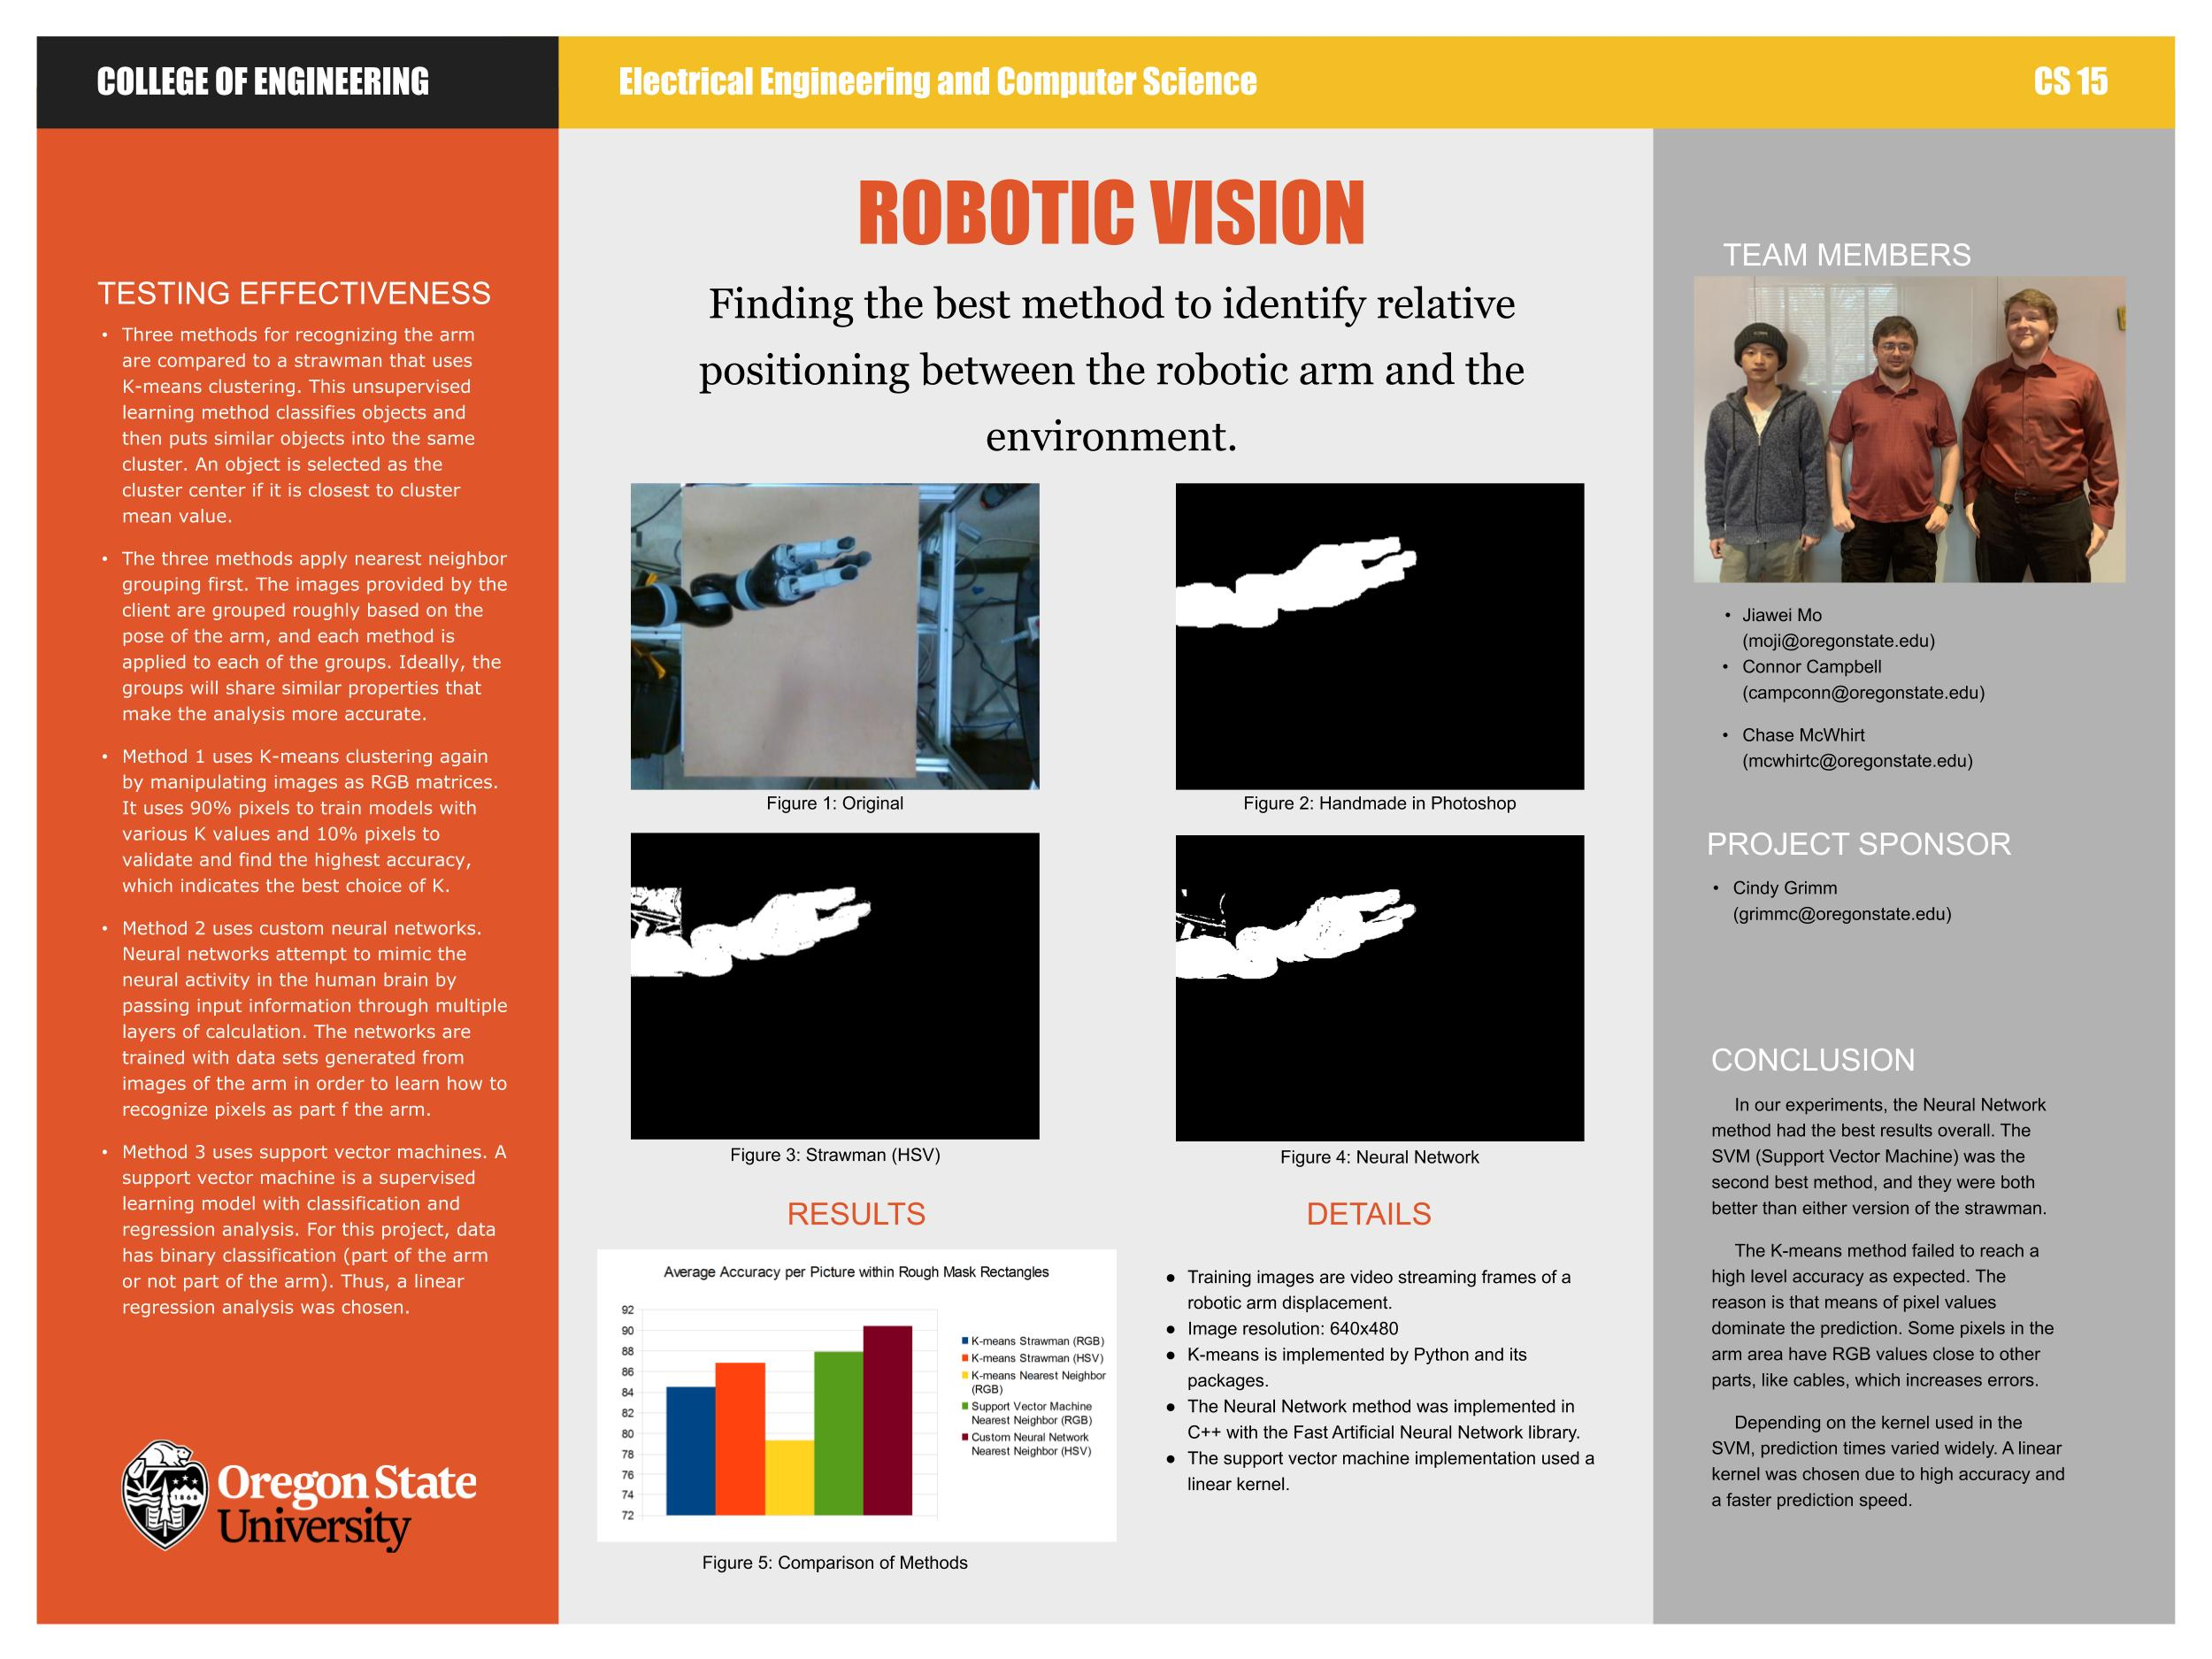
\includegraphics[width=1.\textwidth]{PosterNewDraft.jpg}
  \end{center}
  \caption{Expo Poster}
\end{figure}

\newpage
\section{Project Documentation}
%I.e., user guide, installation guide, or variation on user guide) \\
%---------How does your project work? (Could include the following...) \\
%* What is its structure? \\
%* What is its Theory of Operation? \\
%* Block and flow diagrams are good here. \\

%---------How does one install your software, if any? \\
%---------How does one run it? \\ 
%---------Are there any special hardware, OS, or runtime requirements to run your software? \\
%---------Any user guides, API documentation, etc. \\

%---------This needs to be detailed enough to recreate and/or use your project!
\subsection{Neural Network Guide}

\subsubsection{Structure and Theory}
There are two programs for neural networks: FANN\_Gen and FANN\_Use. FANN\_Gen is use to generate and train neural networks using provided data, while FANN\_Use runs a given neural network over an image to produce a mask. Both of these programs were developed in C++.

\subsubsection{Installation}
The programs were developed in Microsoft Visual Studio, and the simplest way to install them is to open the provided projects in Visual Studio and compile them there. There are a few macros that may be changed in order to utilize old code that experimented with other options, but they are not all stable in the current version, and further changes to the code would be necessary to utilize them.

For FANN\_Gen:
\begin{enumerate}
\item CSV\_DATA \\
If set to 1, uses data from CSVs generated using the createDataSet.py script in Code->Misc. Setting to 0 will cause it to run in image mode, however that was meant for earlier experiments and only scanned a single image whose name was hard coded in.

\item NEW\_NET  \\
If set to 1, the program will generate a new network to train from scratch. If set to 0, the program will load in a preexisting network and continue to train it

\item HSV \\
If set to 1, converts image data to HSV and uses that for training and testing network. If set to 0, uses RGB. This was also meant for earlier experiments, and if RGB is used with CSV\_DATA set to 1, the network will be generated with its outputs reverse relative to what FANN\_Use will be expecting for RGB mode

\item NORMALIZE \\
If set to 1, image values are normalized from -1 to 1. If set to 0, values are used as-is (generally 0 to 255). Recommended to keep at 1.

\item ACC \\
The desired error frequency. If a given set of data is taking too long to train, or can't seem to get to the desired error, this may be adjusted. Be sure to multiply desired error frequency by the number of output nodes (as the code currently is, that would be 2).
\end{enumerate}

For FANN\_Use, the only macro is HSV, which should be set to the same value FANN\_Gen was set to when the network was generated

\subsubsection{Running}
When running FANN\_Gen, two csv files generated by the createDataSet.py script in Code->Misc should be in the same directory: trainingPixels.csv and testingPixels.csv. These files are used for training and testing the network, respectively. The result of the program should be a neural network saved in the file mask.net. If the NEW\_NET macro is set to 0 (it is set to 1 by default), the file mask.net should also be in the directory, presumably generated by a previous running of the program. 

When running FANN\_Use, the image to be analyzed (image.jpeg) and a neural network (mask.net) should be present in the directory. It also takes in 4 command line arguments defining the pixels that should be analyzed in the following order: left-most boundary, top-most boundary, right-most boundary, bottom-most boundary. Anything outside the boundaries will be assumed to be black (ie, not part of the arm). To include the whole picture, enter
\begin{verbatim}
    0 0 640 480
\end{verbatim}

\subsubsection{API Documentation}
\begin{enumerate}
    \item FANN: http://leenissen.dk/fann/wp/
\end{enumerate}

\subsection{Kmeans User Guide}
\subsubsection{Structure and Theory}
The Kmeans model was implemented by Python. Overall, there are three steps. The first one is to process the image sets. Normally, the data will be stored in a matrix data structure. For instance, a matrix [10, 480, 640, 3] represents an image set that has 10 images and each image is 640x480 pixels size with 3 channel including RGB values. The second step is to train the model. Notice that Kmeans is sensitive to data dimension. The matrix that is fed into the Kmeans model can only be 1D or 2D. The last step is to predict images, which will generates masks. By analyzing generated masks, it will tell how the model performs and what parameters need to be tuned to improve this model. In this case, k value is the key parameter that affects the outcome of Kmeans model. It determines the number of clusters of the model. \\

\noindent
Kmeans theory is based on clustering. It aims to put elements of a data set into disjoint clusters, such that samples are self-similar in the same cluster. With a partition of the data into k clusters, a point will be assigned to a cluster if it is closest to that cluster center. After assignment, clusters' centers will be updated by computing the mean coordinates of points of the cluster. While no points are assigned to another cluster, Kmeans clustering will stop.

\subsubsection{Installation}
The model is built up by Python. Version 3.5 is suggested since it is compatible with a lot of packages. The following packages are used in this model:
\begin{enumerate}
\item PIL
\item sklearn
\item matplotlib
\item scipy
\item numpy
\end{enumerate}

\subsubsection{Run}
The model can run on Windows, macOS and Linux. Notice that a Linux system need GPU to visualize graphs and pictures. To run the model, commands should be like this in the terminal, 'python filename.py'. For this model, running 'python kmeans\_10\_test.py' will print out the accuracy. Also, in Visual Studio, pressing Ctrl + F5 to run without debug. 

\subsubsection{Notation}
There are some lines are commented out in python files. They are NOT useless. They are data pre-process and training process. The reason why commenting out them is that this speeds up the program running. The pre-processed data and trained models are saved in .npy files. It is convenient and efficient to reuse them, instead of running the same computation again. If another training is needed, it's better to look through those lines. 


\subsection{Support Vector Machine}
\subsubsection{Structure and Theory}
There are three main scripts that allow the support vector machine to function.
First, there's svmCreate.py, which creates 7 models based on 7 data sets (trainingPixelsGroup[X].csv).
Second, there's svmPredict.py, which makes each respective model create masks from images.
Last, there's svmTest.py, which makes each respective model make predcitions on their test set.

\subsubsection{Installation}
\begin{verbatim}
    Install Python 3.5 (https://www.python.org/downloads/release/python-350/).
    Run this in your preferred command line.
    python -m pip install -U pip matplotlib numpy scikit-learn joblib
\end{verbatim}

\subsubsection{Running}
It's worth noting before running some scripts, configuration is required.
All run commands are expected to be run from the top level directory (Capstone).

\begin{enumerate}
\item svmCreate.py
\begin{verbatim}
    python Code\SVM\svmCreate.py
\end{verbatim}
This creates 7 models from the 7 trainingCSVs located in 'Data/Formatted Pixel Data'.

\item svmTest.py
\begin{verbatim}
    python Code\SVM\svmTest.py
\end{verbatim}
Tests 7 models on the the 7 testingCSVs located in 'Data/Formmatted Pixel Data'.
All output is printed to the commandline.
You can specify an output file (to bash) by adding '> fileName.txt' at the end of the call.

\item svmPredict.py
\begin{verbatim}
    python Code\SVM\svmPredict.py
\end{verbatim}
Will use the 7 models to create 21 predicted masks.
They will always be saved to the 'Support Vector Machine Images' directory.
\end{enumerate}

\subsubsection{Special Hardware}
Special hardware such as GPUs.
Without any multithreading, training takes approximately 8 hours using the linear SVM kernel.
Since everything is in Python 3.5, it runs anywhere that has Python 3.5.

\subsubsection{API Documentation}
\begin{enumerate}
\item SVM (scikit-learn API): https://scikit-learn.org/stable/modules/svm.html

\noindent
\item Saving SVM models (Joblib example): https://scikit-learn.org/stable/modules/model\_persistence.html

\end{enumerate}


\subsection{Semantic Segmentation Convolution Neural Network User Guide}
\subsubsection{Structure and Theory}
This Convolution Neural Network has three basic stages. Similar to Kmeans, it also pre-processes images and then uses matrices to train. Finally, loading the trained model (checkpoints) to predict images, which will generate masks. \\

\noindent
Convolution Neural Network is successful in handling visual, textual and audio data. This network needs to build translation invariance into the model. It ties parameters together in the network and reduces number of parameters. Mostly, it is better than Neural Network since a convolution is robust to objects' position changing in the images. This method allows continual captures of the high level patterns well by sub-sampling.

\subsubsection{Installation}
This model is also implemented by Python3.5 and related packages. In addition, using GPU to train the model will speed it up. Therefore, tools called CUDA and cudnn are needed in order to enable the NVIDIA GPU parallel computation of tensorflow program. It is doable to train with CPU but it would take much time and during the first two trials, the training time was over 30 hours. \\

\noindent
Helpful tools (compatible with GTX1070):
\begin{enumerate}
\item CUDA 10.0
\item cudnn 7.5
\end{enumerate}
\noindent
Needed packages in Python3.5:
\begin{enumerate}
\item tensorflow
\item numpy
\item cv2
\item matplotlib
\item PIL
\end{enumerate}

\subsubsection{Folders and Files Description}
\begin{enumerate}
\item 5\_5\_trial\_1: The first trial. There are checkpoints, accuracy and loss graphs inside.
\item 5\_15\_trial\_2: The second trial. There are checkpoints, accuracy and loss graphs inside.
\item checkpoints: Contains the third trial. Around 180 images are used, containing train, validation, and test. It also has checkpoints and accuracy.
\item images: Contains a gif file, which is compressed by serialized 182 images, combining masks and original images to show effects.
\item pred\_out: The folder that has predicted masks.
\item predict\_them: Has the images that are going to be predicted.
\item Test: Contains test output and a score file that you can see the performance of the test.
\item trial\_3: Has the organized files for training, validation and testing. Inside, class\_dict is using RGB 0, 0, 0 as background and 1, 1, 1 as the robotics arm. You can add other colors to represent other objects.
\item prepare.py: Organize images and labels, like what trial\_3 shows.
\item refine\_mask.py: tune some pixels that are not 0, 0, 0 nor 1, 1, 1.
\item predict.py: To predict an image.
\item test.py: To test an image set.
\item train.py: To train an image set.
\item pred.py: Uses cmd to predict lots of images.
\item combine\_mask.py: Merging masks with original images.
\end{enumerate}

\subsubsection{Running Command}
These statements are also posted in README on github site. Followings are training, validation and testing commands:
\begin{enumerate}
\item python train.py --num\_epochs 250 --checkpoint\_step 6 (6 epoches, 1 checkpoint) --validation\_step 1 (validate for each epoch) --dataset trial\_3 (the folder contains images) --crop\_width 480 --crop\_height 480 --batch\_size 1 --model DeepLabV3 --frontend ResNet101
\item python test.py --checkpoint\_path .\textbackslash checkpoints\textbackslash0080\textbackslash model.ckpt (different directions for different checkpoints) --crop\_height 480 --crop\_width 640 --model DeepLabV3 --dataset trial\_3
\item python pred.py 
\item python predict.py --image 'image path' --checkpoint\_path .\textbackslash checkpoints\textbackslash latest\_model\_DeepLabV3\_trial\_3.ckpt (different directions for different checkpoints) --crop\_height 480 --crop\_width 640 --model DeepLabV3 --dataset trial\_3 
\end{enumerate}

\subsection{``Misc''}
\subsubsection{Structure}
There are four miscellaneous scripts that support each implementation.
First, there's analysis.py which compares two sets of masks (truths versus predictions).
Second, maskToRectangle.py which creates a .csv with two pairs of x,y coordinates from a set of masks.
Third, createDataSet.py creates seven datasets from photos and is how we apply nearest neighbor functionality.
Fourth, is colorPredictionResults.py which acts as a rudamentry prediction method.

\subsubsection{Installation}
\begin{verbatim}
    Install Python 3.5 (https://www.python.org/downloads/release/python-350/).
    Run this in your preferred command line.
    python -m pip install -U pip matplotlib numpy scikit-learn joblib
\end{verbatim}

\subsubsection{Running}
It's worth noting before running some scripts, configuration is required.
All run commands are expected to be run from the top level directory (Capstone).

\begin{enumerate}
\item analysis.py
Configuration required to run analysis.
In order to perform an analysis on your 21 images, you need to edit analysis.py.
Search for '\#\#\# Main'.
Set 'implementationMaskPath' to your folder (containing your 21 predicted masks).
(Note, if you're implementationMaskPath is already available, uncomment it and comment out the active one.)
\begin{verbatim}
    python Code\Misc\analysis.py
\end{verbatim}
Output will be 21 different picture (in the rectangle).
You can dump this into a txt (using Bash) by adding '> fileName.txt' to the bash command.

\item maskToRectangle.py
\begin{verbatim}
    python Code\Misc\maskToRectangle.py
\end{verbatim}
Will analyze the photoshop masks and create a csv containing two (x,y) coordinates and associated file.
The (x,y) coordinates will create a rectangle (inclusive).
This script creates a simulation of the rough masks that we're expecting as input.

\item createDataSet.py
\begin{verbatim}
    python Code\Misc\createDataSet.py
\end{verbatim}
Will create 7 CSVs for training and testing (each).
This is a standard set to be used for the 7 group implementation models.
Essentially, every three images will be collected into one list of dictionaries.
The list will then be shuffled randomly and then split 9:1.
90\% of pixels from the three images will be used for training.
10\% of pixels from the three images will be used for testing.
The random shuffling is currently seeded and will always produce the same output.

\item colorPredictionResults.py
This requires configuration of the cluster size the pixels are sorted into.
\begin{verbatim}
    python Code\Misc\colorPredictionResults.py
\end{verbatim}
Partitions every pixel, based on their RGB values, into clusters.
These clusters then, in a sense, perform a popular vote.
Other pixels that would fall into that cluster would be classed by the popular vote.
(It should also be noted that, while surprisingly accurate, this method is highly overfitted.)
\end{enumerate}

\subsubsection{Special Hardware}
Since everything is in Python 3.5, it runs anywhere that has Python 3.5.

\subsubsection{API Documentation}
\begin{enumerate}
\item NumPy API: https://docs.scipy.org/doc/numpy/index.html

\noindent
\item MatPlotLib API: https://matplotlib.org/

\noindent
\item Python Built-In API: https://docs.python.org/3.5/library/
Built in functions and the libraries csv, sys, os, rand, math were all used.

\end{enumerate}

\newpage
\section{Recommended Technical Resources for Learning More}
%---------What web sites were helpful? (Listed in order of helpfulness.) \\
%---------What, if any, reference books really helped? \\
%---------Were there any people on campus that were really helpful?

\begin{enumerate}

\item API Documentation: \\
https://scikit-learn.org/stable/modules/svm.html \\
https://docs.scipy.org/doc/numpy/index.html \\
https://docs.python.org/3.5/library/ \\
https://scikit-learn.org/stable/modules/model\_persistence.html \\
https://matplotlib.org/ \\
http://leenissen.dk/fann/wp/

\item OpenCV tutorial: https://docs.opencv.org/3.4/d9/df8/tutorial\_root.html 

\item Learning Support Vector Machines: https://youtu.be/\_PwhiWxHK8o

\item Lecture 11 | Detection and Segmentation from Stanford: https://youtu.be/nDPWywWRIRo

\item String Modulo Operator Tutorial: https://www.python-course.eu/python3\_formatted\_output.php

\item Removing large files from .git: https://stackoverflow.com/questions/2100907/how-to-remove-delete-a-large-file-from-commit-history-in-git-repository

\end{enumerate}


\newpage
\section{Conclusions and Reflections}
%---------each team member answers all questions individually
\subsection{Connor}

\subsubsection{What technical information did you learn?}
I've learned quite a bit about neural networks. 
Before joining the project, my experience in them was limited to videos on the internet, which generally either provided more abstract theory, or utilized a relatively niche version. 
I was under the impression that using a genetic algorithm to train a network was common, since many of the videos dealt with video games, which required flexible structures that didn't necessarily know the best possible output at any given time. 
During the tech review, I quickly realized that that was essentially the only time such a method would ever be used and that back propagation was the preferred method for almost any other scenario.


\subsubsection{What non-technical information did you learn?}
I learned a lot about myself and my work ethic. 
It was really hard to motivate myself to work when I didn't have a set schedule of what times to sit down and get stuff done. 
Before this year, I had considered finding a job where I could work from home, but now I think that I benefit a lot from having a specific time and place to be in for working.

As a side note, I also got some experience in writing technical documents.

\subsubsection{What have you learned about project work?}
Planning ahead is incredibly important. 
Not only in what needs to be done, but in when to get certain parts done. 
It can be hard to feel motivated when you have a vague idea of what needs to be done over a long period of time, so it's useful to have smaller, discrete, incremental goals. 
There were times when I had a specific idea of what I needed to get done and when, and I was able to work hard and quickly at those points, but if I wasn't sure exactly what I needed to do, or if the next thing to do was a ways away when I had other homework, it was easy to lose track of myself.


\subsubsection{What have you learned about project management?}
I went over this in the previous section: smaller, discrete goals over shorter periods of time are easier to focus on.


\subsubsection{What have you learned about working in teams?}
It can be frustrating.
Before elaborating, I want to be absolutely clear that this is by no means the fault of my co-workers.
I found that I'm a lot better at communicating in person than over the internet.
When we met in person, I felt more confident in saying what I wanted or needed to say and participating in the conversation, but online, I had a tendency to type slowly or be too concerned with my exact phrasing or sending a message in the middle of a conversation, that I often ended up being a lot quieter than I wanted to be.
Also, I've always had trouble taking initiative in group projects, and I think that was a major weakness of mine, especially early on when we were all unfamiliar with each other and still unsure about certain parts of the project.


\subsubsection{If you could do it all over, what would you do differently?}

If I'm honest, there were times when I thought I would've been happier taking on a different project. 
When I was told to pick projects based on interest rather than familiarity, I ended up signing up for something I knew almost nothing about. 
I wouldn't have wanted something trivial, but something I'm a little more familiar with probably would have gone more smoothly.

As for this project on its own, the first thing that comes to mind would be taking more initiative early on, and trying to be more organized. 
Like I said for the project work section, I probably would have been more focused overall if I had defined more specific goals and time frames for my parts of the project. 


\subsection{Chase McWhirt}
\subsubsection{What technical information did you learn?}
I learned a lot about Python, which was one of my weakest languages.
After working it more, I've come to appreciate it as a language.
I learned how to implement a support vector machine.
Eventually, I also learned what it actually was and how to distinquish it from the other implementations.
Going more fine grain, I learned about various APIs, how they interact, and why they're fairly popular in machine learning applications.
I also practiced some version control and data interpretation mechanics I already knew.

\subsubsection{What non-technical information did you learn?}
I learned the value of standing up for myself.
At Expo, I had to practice taking some pride in a project I put a lot of work into, even if it can be difficult to define the value or magnitude of the project.
I learned to manage many different parts of the project.
I also learned to delegate instead of letting those pieces destroy me.

\subsubsection{What have you learned about project work?}
Project work can often times be rewarding.
The rewards of cooperation are often more work being completed and a more well rounded project.
It has its downsides as well.
In some ways, it can be less efficient.
Thus, you often have to take intiative in a variety of ways to mitigate those inefficiencies.

\subsubsection{What have you learned about project management?}
You can't force a workflow on a project.
Some workflows also aren't always the best fit for a project.
For example, I spent a lot of time creating a bunch of commits and comments regarding program functionality.
However, this was a redundant exercise as the project was split into many divisions and the group never had to work on each others' code.
In this scenario, I learn to take on more than I could handle, and then delegate when applicable.
This came up the most often in written portions as fall term was spent designing and dividing the project into equal parts.
In a sense, I learned to manage up and across.

\subsubsection{What have you learned about working in teams?}
It is extremely difficult to divide work equally among a team.
Often, the best approach is to divide work such that everyone does what they're good at.
For example, if there are two people on a team, and they have a code assignment and a writing assignment, it's better to give one the code assignment and the other the writing assignment.
If you split the code in half and the writing in half, if one person is better at writing and the other at coding, they'll feel as if underperforming in their weak areas.
Ironically, doing the easiest pieces for yourself often makes the group more productive, as long as there's variance in specialty.

\subsubsection{If you could do it all over, what would you do differently?}
I genuinely don't know what I would do differently.
It's inevitable that despite setting requirements early and thoroughly, there will be pressure to change them and/or ignore them entirely.
In a way, it makes you feel as if the best answer is to spend more time defining requirements.
However, after a certain point, it becomes pointless and redundant to do such.
Honestly, the best piece of insight I got was from my boss.
To paraphrase, it's best to ask specific questions rather to over promise.
In a sense, abstract clients out of the development process as much as possible.
For a related example, imagine a person is tasked with redesigning a car.
They ask drivers what there biggest complaints are about driving the current model of car.
They respond that it doesn't accelerate fast enough, it has a bad stereo, and that the cup holders are too small.
The designer creates a new model of the car.
It has a better stereo and the cup holders securely hold 7-11 Big Gulps.
Drivers are much more likely to be satisfied with this new model rather than disappointed the acceleration remained unchanged.
In this sense, I wish I had picked a project I knew well enough already that I wouldn't need to rely on guidance from the client.
In a way, I let the popularity of machine learning draw me towards this project when I likely could have done other projects and learn just as much without some of the struggles I had with this project.


\subsection{Jiawei Mo}
\subsubsection{What technical information did you learn?}
I have learned that Kmeans algorithm is not robust to noise. This is noticeable by evaluating the masks generated by Kmeans model. The same as Support Vector Machine, it has shown an ideal performance in hand written numbers prediction. However, the robotics arm images have more complicated features. Thus, the prediction masks also show noise pixels. Neural Network is better comparing to previous models since it can add nodes for more weight parameters but the arm is moving, which leads to an issue that the arm pixels will be fed into another weight parameters since its position (coordinates) is changed in the images. This problem is fixed by adding a convolution to Neural Network, which matches the expectation that Convolution Neural Network performs better. It has around 98.5\% accuracy on testing sets.

\subsubsection{What non-technical information did you learn?}
The object recognition problem by using image sets is a math problem. Not like perception of human beings, a computer only treat things as data, including images, voices or words. The tools that I used to process digital data were vector, matrix, projection, convolution. They all are mathematical tools. I would claim that high level of math skills are required in order to solve a problem by implementing Machine Learning and Deep Learning models.

\subsubsection{What have you learned about project work?}
I found that project work is like a delicate machine. Since this project is a subtask of a big project, each group is related to other groups. There are teams that work on robotics arm building, materials testing and also programming. One obstacle that our group had met was that the training images were delayed for few weeks because of a trouble of arm moving video stream capture. This shows that even a little segment issue would impact whole project. 

\subsubsection{What have you learned about project management?}
I have learned that preparation is also important. It contains specific knowledge researches and useful techniques review. With understanding of the project problems and knowing different kinds of solutions, I could be more confident to come up a blueprint of the project. As some Tech Reviews depict, I could evaluate potential performance and cost of solutions.

\subsubsection{What have you learned about working in teams?}
I found that information sharing makes team work more efficient. It is a fact that people cannot remember all details and know about skills in any field. However, by working as a group, teammates can sharing information that others don't have. I remembered that I pointed out OpenCV and Conner could use this to pre-process our training images. For instance, program is not using RGB order to store pixels and this could help Conner to solve problems. Also, I introduced Serialization packages to Chase and then he can use this technique to store trained models for trials with different parameters.

\subsubsection{If you could do it all over, what would you do differently?}
If I could do it all over, I would advise our client that a Convolution Neural Network would be a better choice to deal with this problem. Therefore, we can use this method to improve performance right after Kmeans, SVM and Neural Network trials. Before the beginning of the implementation, I had reviewed some paper that indicated high performance of image recognition by using Convolution Neural Network. This was what I used in the end of this term to produce a good mask.

\newpage
\section{Appendix}
\subsection{Appendix 1: Essential Code Listings}

\subsubsection{Preparing and Generating Neural Networks with FANN}
The code for generating networks with FANN is actually rather simple. Once you have your network set up, you read in data from a file, train it, and test its effectiveness on the test data. There are several variables and options that could be changed when setting up the network. Below are a few settings that were experimented with:

\begin{verbatim}
	const float learning_rate = 0.7f;
	const unsigned int num_layers = 5;
	const unsigned int num_input = 3;
	const unsigned int num_hidden = 4;
	const unsigned int num_output = 2;

	net.create_standard(num_layers, num_input, num_hidden, num_hidden, num_hidden, num_output);

	net.set_learning_rate(learning_rate);

	net.set_activation_steepness_hidden(1.0);
	net.set_activation_steepness_output(1.0);

	net.set_activation_function_hidden(FANN::SIGMOID_SYMMETRIC_STEPWISE);
	net.set_activation_function_output(FANN::SIGMOID_SYMMETRIC_STEPWISE);

	net.set_train_stop_function(FANN::STOPFUNC_BIT);
\end{verbatim}

In particular, the structure of the network (number of layers and number of nodes per layer) has a big effect on the accuracy, training time, and whether it is over-fitted. The train stop function line indicates that accuracy was determined based on how many output nodes gave a response outside an accepted range, as oppose to the default, where accuracy is determined by how different the response was from the desired value.



\subsubsection{Scikit-Learn Support Vector Machines}
The core code that you have to understand is actually available directly in the API documentation.
To create a model for classification, most machine learning algorithms take two inputs.
X in the copied example is a vector of data samples with the dimensions [m-samples, n-features].
y is a vector of classes (as in classifications, not object classes) with dimension [m-samples].
This sample can be practiced directly in a Python terminal.
\begin{verbatim}
    >>> from sklearn import svm
    >>> X = [[0, 0], [1, 1]]
    >>> y = [0, 1]
    >>> clf = svm.SVC(gamma='scale')
    >>> clf.fit(X, y)  
    SVC(C=1.0, cache_size=200, class_weight=None, coef0=0.0,
        decision_function_shape='ovr', degree=3, gamma='scale', kernel='rbf',
        max_iter=-1, probability=False, random_state=None, shrinking=True,
        tol=0.001, verbose=False)
\end{verbatim}
In Python, the $>>>$ represents terminal input.
We can see that with their X and y, they have two data points with two features.
Data point [0, 0] has class 0 while data point [1, 1] has class 1.
It's also extremely important to ensure quality in loading your data before you start ``fitting'' a model.
Even more importantly, you should have a way to save your model, either with data serialization, or another method, or else you'll have wasted time with this much code.

After you've saved your model for repeated uses, you can make predictions.
\begin{verbatim}
    >>> clf.predict([[2., 2.]])
    array([1])
\end{verbatim}
Understanding this code structure is critical to building a support vector machine (but not necessarily understanding support vector machines themselves).
As an exercise, why do you think making a class prediction of [2, 2] yielded class 1 and not 0?

\subsubsection{Kmeans - Flatten Matrix}
Moreover, it is important to flatten the high dimensional matrix as a one dimension array structure. The reason is that the K-means algorithm can only work on the one dimension or two dimension data structure. The process of jpeg.reshape below will return a one dimension array and every single element represents a pixel value. It can be arbitrary value of RGB. 

\begin{verbatim}
jpeg_feed = jpeg.reshape(jpeg.shape[0] * jpeg.shape[1] * jpeg.shape[2] * jpeg.shape[3], 1)
\end{verbatim}

\subsubsection{Kmeans - Predict}
The main process of K-means algorithm is to create a mask of the original data. By setting number of clusters and predicting the images, we received the mask stored in the variable, result. Its elements were integers from 0 to 3. After reshaping it to image matrix, we could show this mask and save it to the driver. 

\begin{verbatim}
n_clusters = 4
kmeans = KMeans(n_clusters=n_clusters, random_state=0).fit(jpeg_feed)
result = kmeans.predict(jpeg_feed)
result = result.reshape(21, 480, 640, 3)
\end{verbatim}



\subsection{Appendix 2: Photos}
\begin{figure}[H]
  \begin{center}
    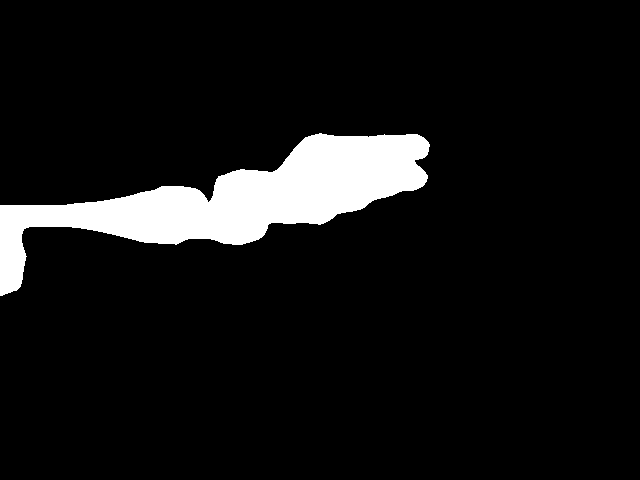
\includegraphics[width=1.\textwidth]{1548556288818083016_pred.png}
  \end{center}
  \caption{A Mask Generated by Semantic-Segmentation CNN without Rectangle Refining}
\end{figure}

\begin{figure}[H]
  \begin{center}
    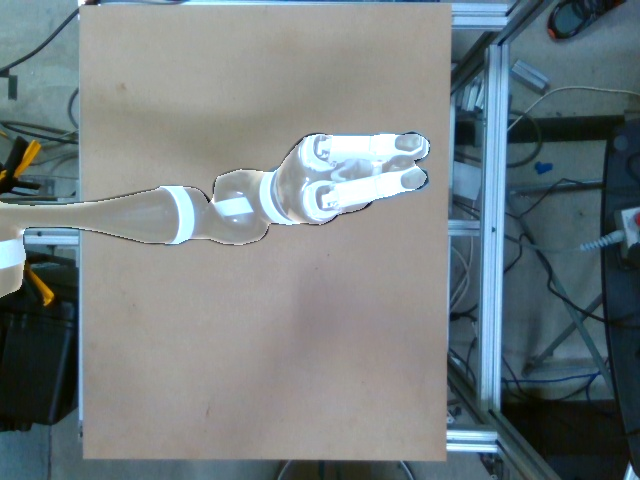
\includegraphics[width=1.\textwidth]{combined_112.png}
  \end{center}
  \caption{A Sample of Semantic-Segmentation CNN: Combination of Original Picture and Generated Mask without Rectangle Refining}
\end{figure}

\newpage
% bibliography
\nocite{*}%if nothing is referenced it will still show up in refs
\bibliographystyle{ieeetr}
\bibliography{refs}
%end bibliography
\end{document}